\part{Lecture 01: Introduction to Reinforcement Learning}
\title[RL Lecture 01]{Lecture 01: Introduction to Reinforcement Learning}  
\date{}  
\frame{\titlepage} 
\frame{\frametitle{Table of contents}\tableofcontents} 

%%%%%%%%%%%%%%%%%%%%%%%%%%%%%%%%%%%%%%%%%%%%%%%%%%%%%%%%%%%%%%%%%%
\section{Course framework} 
%%%%%%%%%%%%%%%%%%%%%%%%%%%%%%%%%%%%%%%%%%%%%%%%%%%%%%%%%%%%%%%%%%

%%%%%%%%%%%%%%%%%%%%%%%%%%%%%%%%%%%%%%%%%%%%%%%%%%%%%%%%%%%%%
%% Teaching team %%
%%%%%%%%%%%%%%%%%%%%%%%%%%%%%%%%%%%%%%%%%%%%%%%%%%%%%%%%%%%%%
\begin{frame}
\frametitle{The teaching team}
\vspace{-0.5cm}
\begin{columns}[t]

	\column[T]{0.16\textwidth}
	\begin{figure}
		\centering
			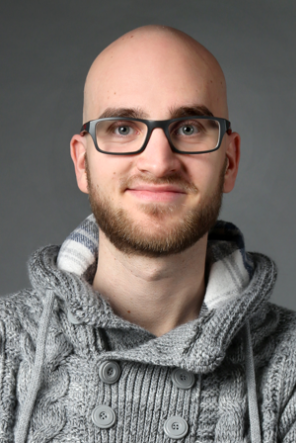
\includegraphics[height=3cm]{fig/lec01/Jakobeit.png}
			\caption*{Darius \\Jakobeit}
	\end{figure}
			
	\column[T]{0.16\textwidth}
	\begin{figure}
		\centering
			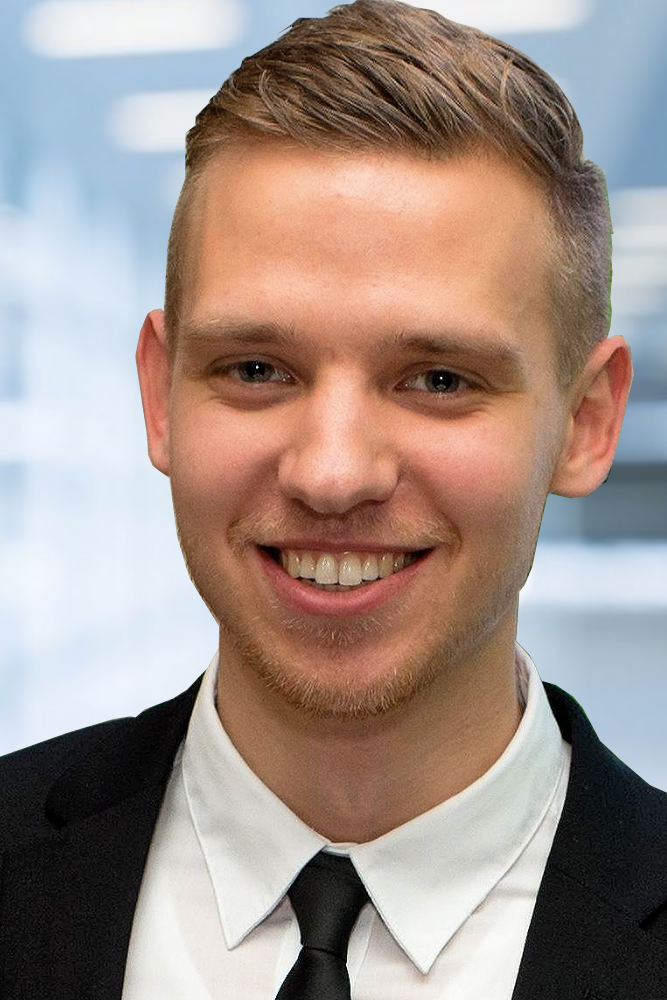
\includegraphics[height=3cm]{fig/lec01/Kirchgaessner.png}
			\caption*{Wilhelm Kirchg�ssner}
	\end{figure}
	
	\column[T]{0.16\textwidth}
	\begin{figure}
		\centering
			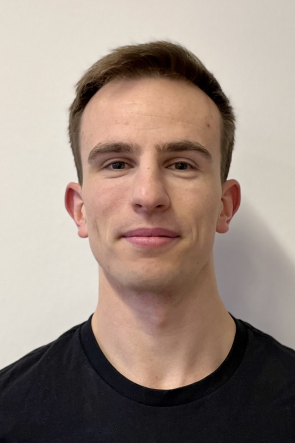
\includegraphics[height=3cm]{fig/lec01/Meyer.png}
			\caption*{Marvin \\Meyer}
	\end{figure}
	
	\column[T]{0.16\textwidth}
	\begin{figure}
		\centering
			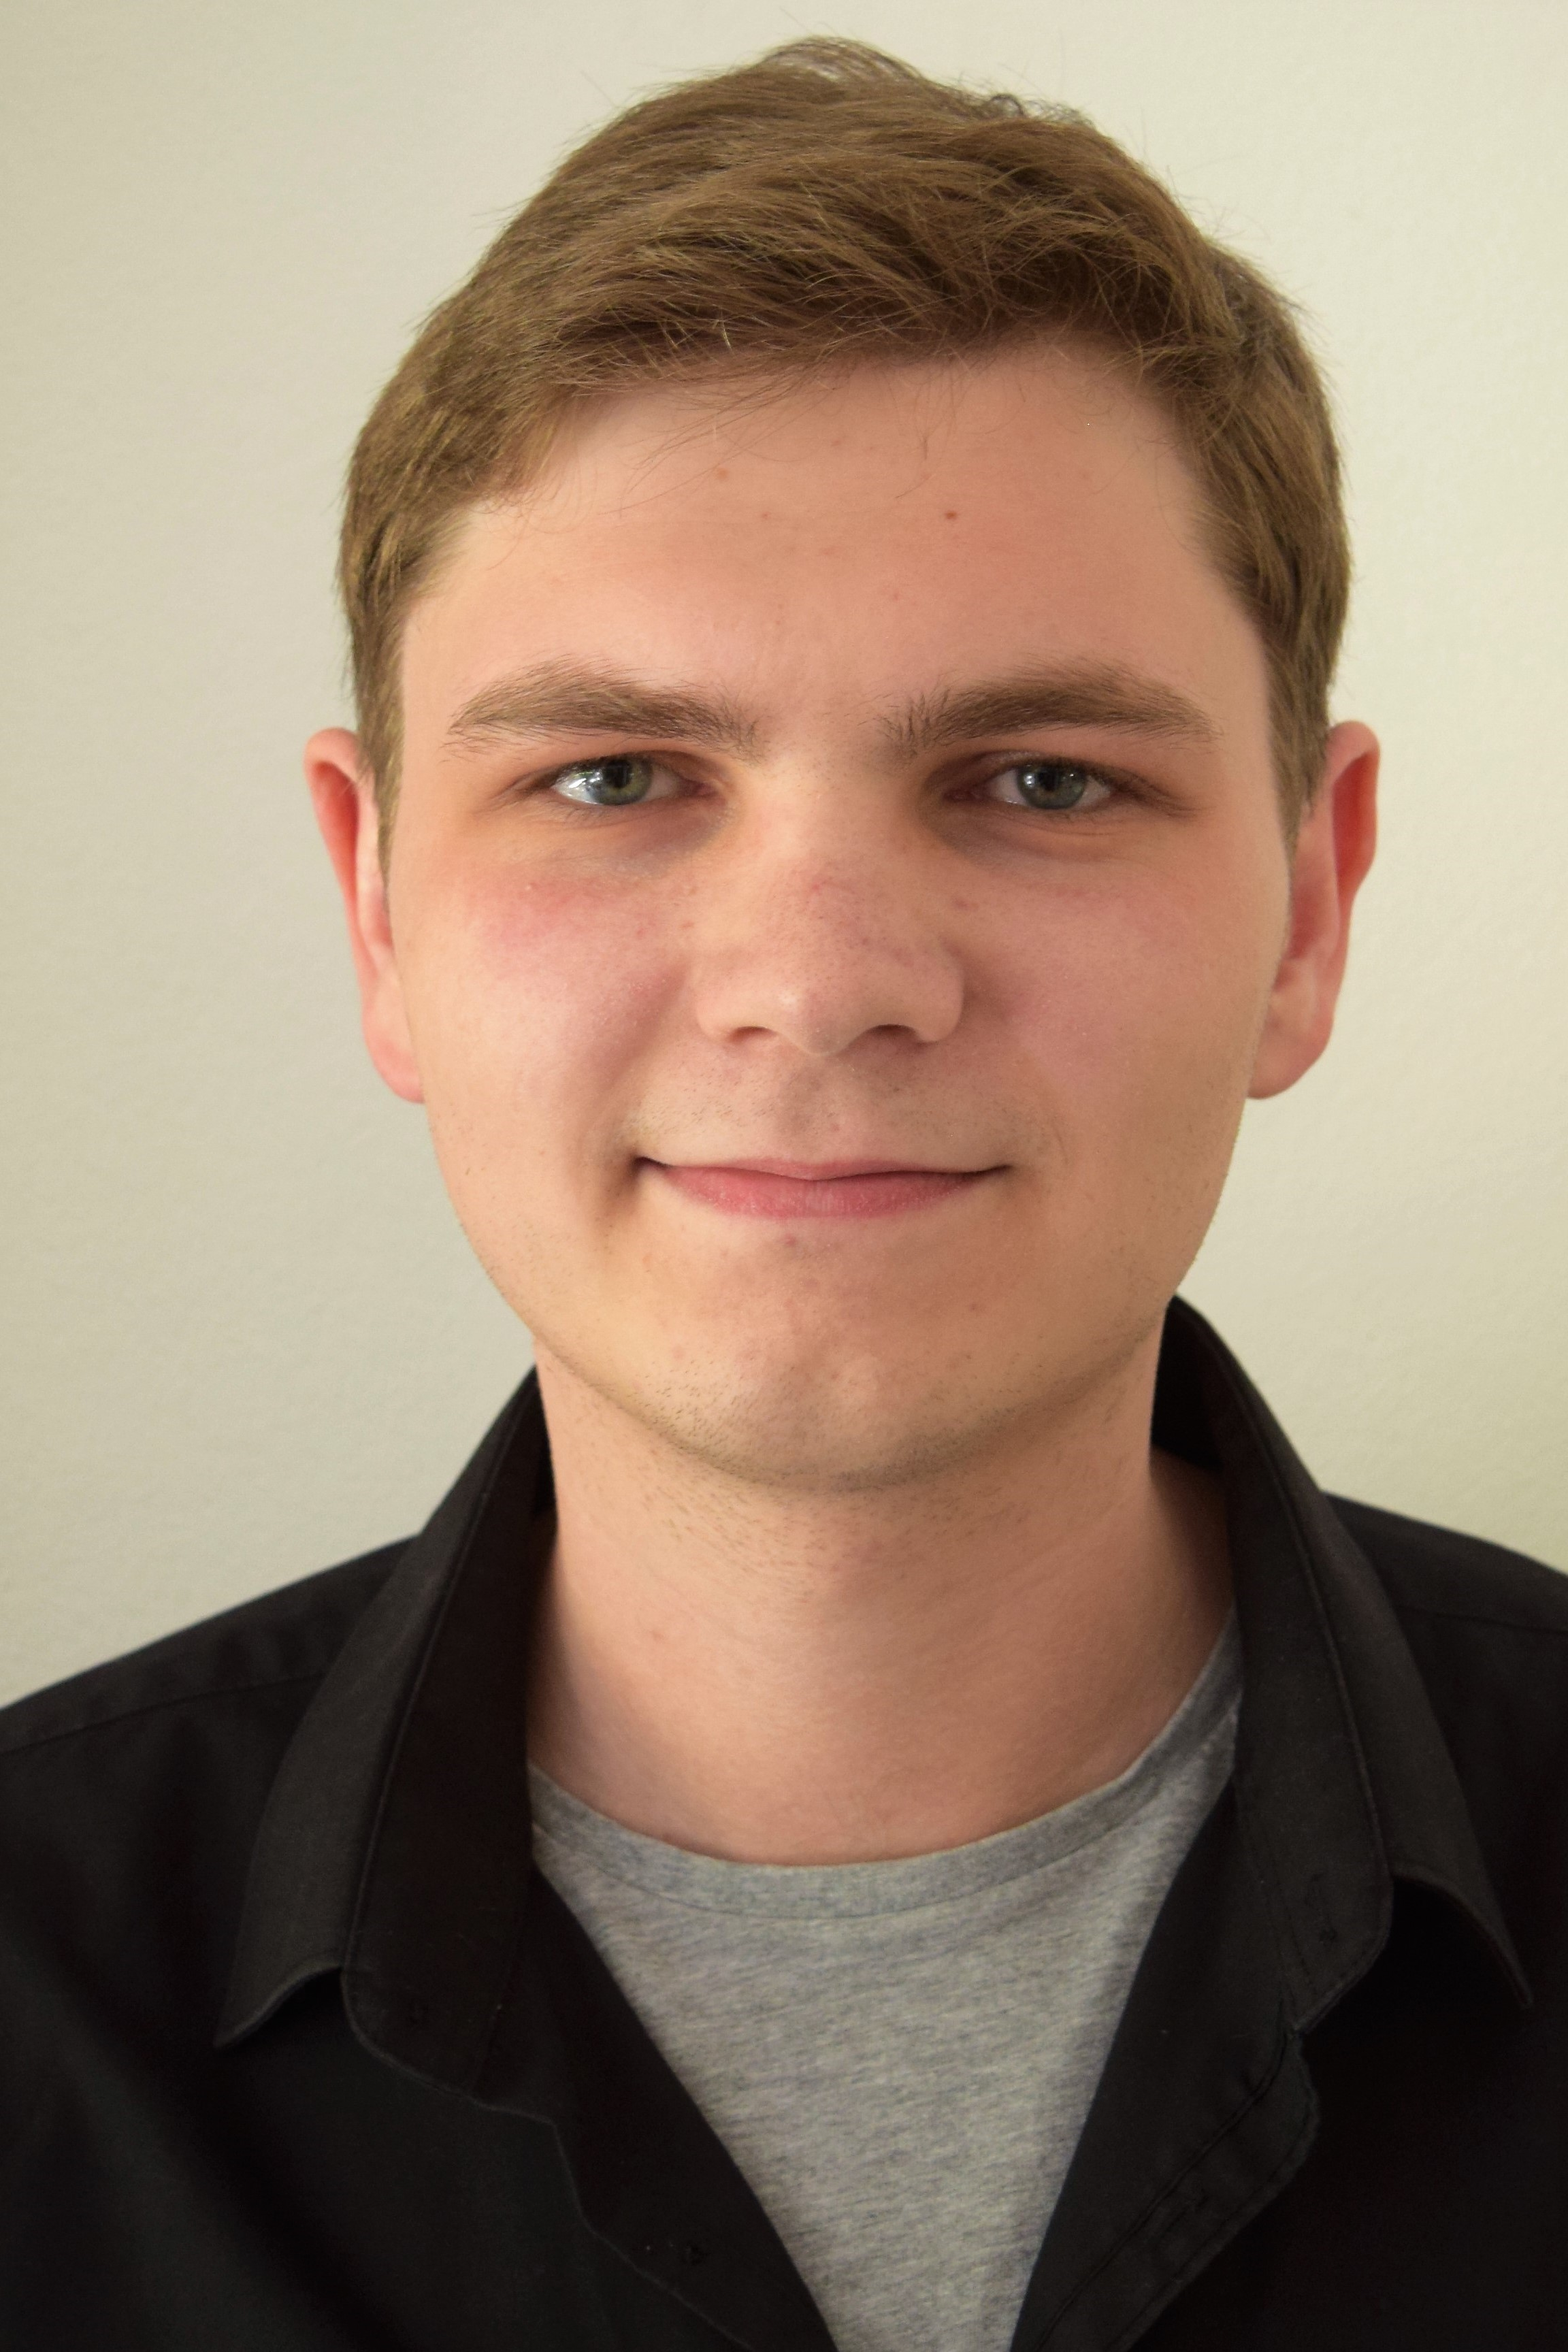
\includegraphics[height=3cm]{fig/lec01/Schenke.jpg}
			\caption*{Maximilian Schenke}
	\end{figure}
	
	\column[T]{0.16\textwidth}
	\begin{figure}
		\centering
			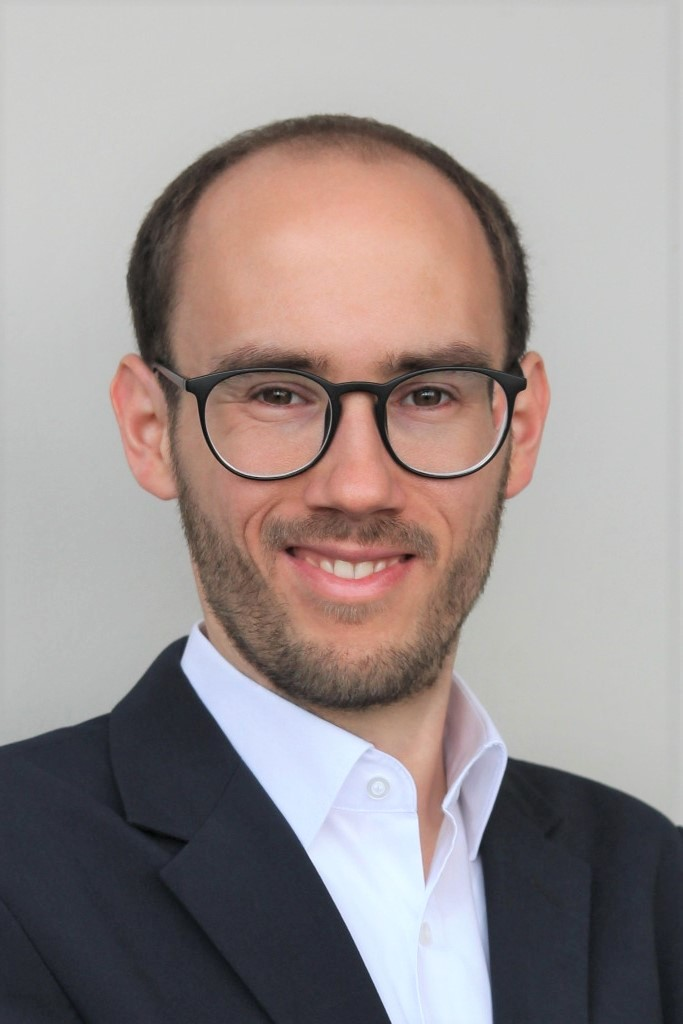
\includegraphics[height=3cm]{fig/lec01/Wallscheid.jpg}
			\caption*{Oliver\\ Wallscheid}
	\end{figure}
	
	\column[T]{0.16\textwidth}
	\begin{figure}
		\centering
			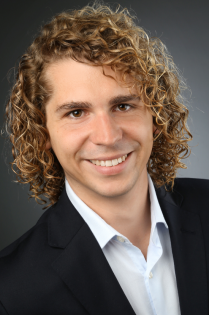
\includegraphics[height=3cm]{fig/lec01/Weber.png}
			\caption*{Daniel\\ Weber}
	\end{figure}
\end{columns}
\vspace{-0.25cm}
\begin{block}{Contact}
	\begin{itemize}
		\item Email: \href{mailto:wallscheid@lea.upb.de; weber@lea.upb.de; kirchgaessner@lea.upb.de; schenke@lea.upb.de; jakobeit@lea.upb.de; meyer@lea.upb.de}{\{jakobeit, kirchgaessner, meyer, schenke, wallscheid, weber\}$@$lea.upb.de}
		\item Offices: E-building, 4th floor
		\item Individual appointments on request (remote or personally)
	\end{itemize}
\end{block}
\end{frame}

%%%%%%%%%%%%%%%%%%%%%%%%%%%%%%%%%%%%%%%%%%%%%%%%%%%%%%%%%%%%%
%% Examination Regulations %%
%%%%%%%%%%%%%%%%%%%%%%%%%%%%%%%%%%%%%%%%%%%%%%%%%%%%%%%%%%%%%
\begin{frame}
\frametitle{Examination Regulations}
\begin{block}{Final exam}
\begin{itemize}
	\item Oral examination 
	\item Average 45 minutes for presentation and discussion
	\item Individual appointment request via email (at least 2 weeks in advance)
\end{itemize}
\end{block}
\pause
\begin{block}{Pre-exam homework assignment}
\begin{itemize}
	\item Made available via Panda at end of the lecture series.
	\item Practical RL programming task, i.e., solve a typical RL problem.
	\item Further regulations:
	\begin{itemize}
		\item Submit your final programming solution via Panda at least two days before the exam.
		\item Prepare a concise, high-quality presentation to be given at the exam start (roughly 10 minutes). Analyze and evaluate your own results critically. 
	\end{itemize}
\end{itemize}
\end{block}
\end{frame}

%%%%%%%%%%%%%%%%%%%%%%%%%%%%%%%%%%%%%%%%%%%%%%%%%%%%%%%%%%%%%
%% Course Outline %%
%%%%%%%%%%%%%%%%%%%%%%%%%%%%%%%%%%%%%%%%%%%%%%%%%%%%%%%%%%%%%
\begin{frame}
\frametitle{Course outline}
The course will cover the following content:
\vspace{0.25cm}
\begin{itemize}
		\item Conceptual basics and historical overview \pause
		\item Markov decision processes \pause
		\item Dynamic programming \pause
		\item Monte Carlo learning \pause
		\item Temporal difference learning \pause
		\item Bootstrapping \pause
		\item Planning \pause  
		\item Function approximation and deep learning \pause
		\item Eligibility traces \pause
		\item Policy gradient methods \pause
		\item Contemporary (deep) RL algorithms
	\end{itemize}
\end{frame}

%%%%%%%%%%%%%%%%%%%%%%%%%%%%%%%%%%%%%%%%%%%%%%%%%%%%%%%%%%%%%
%% Textbooks %%
%%%%%%%%%%%%%%%%%%%%%%%%%%%%%%%%%%%%%%%%%%%%%%%%%%%%%%%%%%%%%
\begin{frame}
\frametitle{Recommended textbooks}
\begin{itemize}
		\item Reinforcement learning: an introduction, 
		\begin{itemize}
			\item R. Sutton and G. Barto
			\item MIT Press, 2nd edition, 2018
			\item Available \href{http://www.incompleteideas.net/book/the-book.html}{here}
		\end{itemize}
		\vspace{0.5cm}
		\pause
		\item Reinforcement learning (lecture script)
		\begin{itemize}
		  \item D. Silver
			\item Entire slide set available \href{https://www.davidsilver.uk/teaching/}{here}
			\item YouTube lecture series (click \href{https://www.youtube.com/watch?v=2pWv7GOvuf0}{here})
		\end{itemize}
		\vspace{0.5cm}
		\pause
		\item Reinforcement learning and optimal control
		\begin{itemize}
			\item D. Bertsekas
			\item Athena Scientific, 2019
			\item Available in library
		\end{itemize}
		
	\end{itemize}
\end{frame}


%%%%%%%%%%%%%%%%%%%%%%%%%%%%%%%%%%%%%%%%%%%%%%%%%%%%%%%%%%%%%
\section{Reinforcement learning: what is it?} 
%%%%%%%%%%%%%%%%%%%%%%%%%%%%%%%%%%%%%%%%%%%%%%%%%%%%%%%%%%%%%

\begin{frame}
\frametitle{Table of contents}
\tableofcontents[currentsection]
\end{frame}

%%%%%%%%%%%%%%%%%%%%%%%%%%%%%%%%%%%%%%%%%%%%%%%%%%%%%%%%%%%%%
%% RL Wiki Optimization Cricle %%
%%%%%%%%%%%%%%%%%%%%%%%%%%%%%%%%%%%%%%%%%%%%%%%%%%%%%%%%%%%%%
\frame{\frametitle{The basic reinforcement learning structure}
\begin{columns}[t,onlytextwidth]
\begin{column}{0.6\textwidth}
\begin{minipage}[c]{\linewidth}
	\begin{figure}
		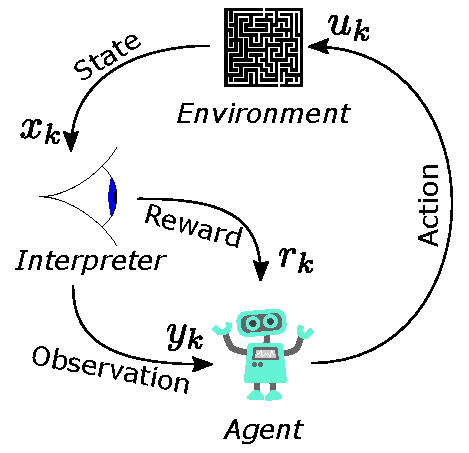
\includegraphics[height=0.6\textheight]{fig/lec01/RL_Wiki.pdf}
		\caption{The basic RL operation principle\\(derivative of \href{https://commons.wikimedia.org/wiki/File:Reinforcement_learning_diagram.svg}{www.wikipedia.org}, \href{https://creativecommons.org/publicdomain/zero/1.0/deed.en}{CC0 1.0})}
		\label{fig:RL_Wiki}
	\end{figure}
\end{minipage}
\end{column}
\hfill
\begin{column}{0.38\textwidth}
\begin{minipage}[c]{\linewidth}
\vspace{0.3cm}
Key characteristics:
	\begin{itemize}
		\item No supervisor
		\item Data-driven
		\item Discrete time steps
		\item Sequential data stream (not i.i.d. data)
		\item Agent actions affect subsequent data (sequential decision making)
	\end{itemize}
\end{minipage}
\end{column}
\end{columns}
\blfootnote{The nomenclature of this slide set is based on the default variable usage in control theory. In other RL books, one often finds $s$ as state, $a$ as action and $o$ as observation.}
}

%%%%%%%%%%%%%%%%%%%%%%%%%%%%%%%%%%%%%%%%%%%%%%%%%%%%%%%%%%%%%
%% Agent and Environment %%
%%%%%%%%%%%%%%%%%%%%%%%%%%%%%%%%%%%%%%%%%%%%%%%%%%%%%%%%%%%%%
\frame{\frametitle{Agent and environment}
\begin{minipage}[t]{0.5\linewidth}
	\begin{figure}
		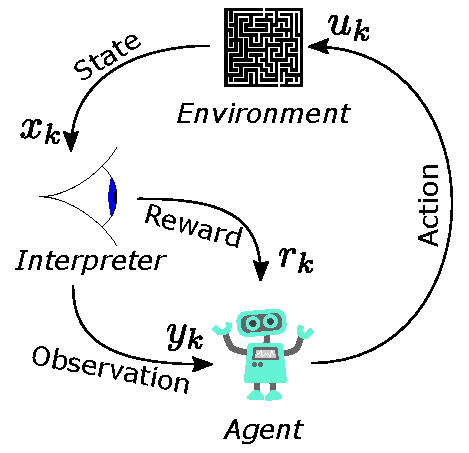
\includegraphics[height=0.55\textheight]{fig/lec01/RL_Wiki.pdf}
	\end{figure}
\end{minipage}
\hfill
\begin{minipage}[t]{0.48\linewidth}

At each step $k$ the agent:
	\begin{itemize}
		\item Picks an action $u_k$.
		\item Receives an observation $y_k$.
		\item Receives a reward $r_k$.
	\end{itemize}
\pause
At each step $k$ the environment:
	\begin{itemize}
		\item Receives an action $u_k$.
		\item Emits an observation $y_{k+1}$.
		\item Emits a reward $r_{k+1}$.
	\end{itemize}
The time increments $k \leftarrow k+1$.	
\end{minipage}
\pause
\begin{block}{Remark on time}
A one step time delay is assumed between executing the action and receiving the observation as well as reward. We assume that the resulting time interval $\Delta t = t_k - t_{k+1}$ is constant.
\end{block}
}

%%%%%%%%%%%%%%%%%%%%%%%%%%%%%%%%%%%%%%%%%%%%%%%%%%%%%%%%%%%%%
%% What is Learning? %%
%%%%%%%%%%%%%%%%%%%%%%%%%%%%%%%%%%%%%%%%%%%%%%%%%%%%%%%%%%%%%
\frame{\frametitle{Some basic definitions from the literature}
What is reinforcement?
\begin{itemize}
	\item ``\textit{Reinforcement is a consequence applied that will strengthen an organism's future behavior whenever that behavior is preceded by a specific antecedent stimulus.[...]There are four types of reinforcement: positive reinforcement, negative reinforcement, extinction, and punishment.}'', \href{https://en.wikipedia.org/wiki/Reinforcement}{wikipedia.org} (obtained 2023-03-31) 
\end{itemize}
\pause
\vspace{0.5cm}
What is learning?
\begin{itemize}
	\item ``\textit{Acquiring knowledge and skills and having them readily available from memory so you can make sense of future problems and opportunities.}'', From Make It Stick: The Science of Successful Learning, Brown et al., Harvard Press, 2014
\end{itemize}
}

%%%%%%%%%%%%%%%%%%%%%%%%%%%%%%%%%%%%%%%%%%%%%%%%%%%%%%%%%%%%%
%% RL vs. (un-)supervised learning %%
%%%%%%%%%%%%%%%%%%%%%%%%%%%%%%%%%%%%%%%%%%%%%%%%%%%%%%%%%%%%%
\frame{\frametitle{Context around reinforcement learning}
\begin{figure}
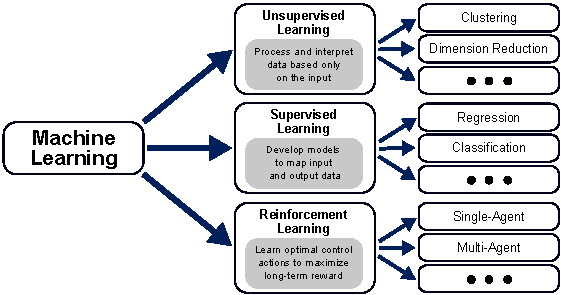
\includegraphics[height=0.7\textheight]{fig/lec01/Machine_Learning_Disciplines.pdf}
\caption{Disciplines of machine learning}
\label{fig:Machine_Learning_Disciplines}
\end{figure}
}

%%%%%%%%%%%%%%%%%%%%%%%%%%%%%%%%%%%%%%%%%%%%%%%%%%%%%%%%%%%%%
%% Context Around Machine Learning %%
%%%%%%%%%%%%%%%%%%%%%%%%%%%%%%%%%%%%%%%%%%%%%%%%%%%%%%%%%%%%%
\frame{\frametitle{Context around machine learning}
\begin{figure}
\centering
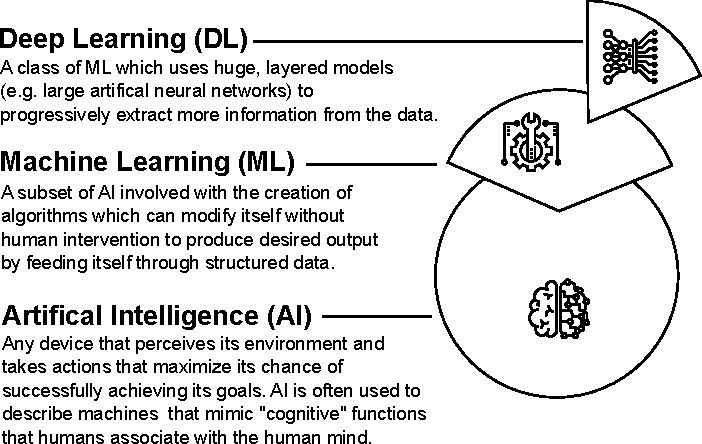
\includegraphics[height=0.7\textheight]{fig/lec01/ML_AI.pdf}
\caption{The broader scope around machine learning}
\label{fig:ML_AI}
\end{figure}
}

%%%%%%%%%%%%%%%%%%%%%%%%%%%%%%%%%%%%%%%%%%%%%%%%%%%%%%%%%%%%%
%% Many Faces of Reinforcement Learning (D.Silver) %%
%%%%%%%%%%%%%%%%%%%%%%%%%%%%%%%%%%%%%%%%%%%%%%%%%%%%%%%%%%%%%
\frame{\frametitle{Many faces of reinforcement learning}
\begin{figure}
\centering
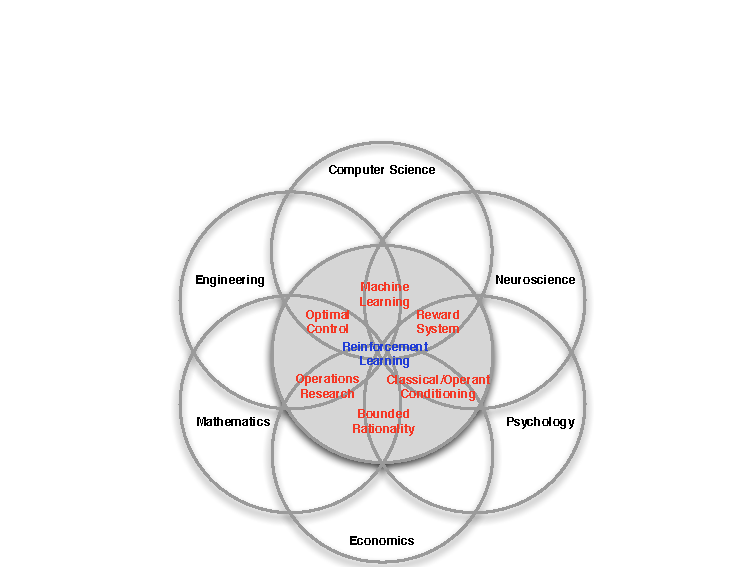
\includegraphics[height=0.7\textheight]{fig/lec01/Faces_RL.pdf}
\caption{RL and its neighboring domains\\ \SilverLectureSource}
\label{fig:Faces_RL}
\end{figure}
}

%%%%%%%%%%%%%%%%%%%%%%%%%%%%%%%%%%%%%%%%%%%%%%%%%%%%%%%%%%%%%%%%%%
\section{Application examples and historic review} 
%%%%%%%%%%%%%%%%%%%%%%%%%%%%%%%%%%%%%%%%%%%%%%%%%%%%%%%%%%%%%%%%%%
\begin{frame}
\frametitle{Table of contents}
\tableofcontents[currentsection]
\end{frame}

%%%%%%%%%%%%%%%%%%%%%%%%%%%%%%%%%%%%%%%%%%%%%%%%%%%%%%%%%%%%%
%% Methodical origins %%
%%%%%%%%%%%%%%%%%%%%%%%%%%%%%%%%%%%%%%%%%%%%%%%%%%%%%%%%%%%%%
\frame{\frametitle{Methodical origins}
\begin{minipage}[t]{0.27\linewidth}
	\begin{figure}
		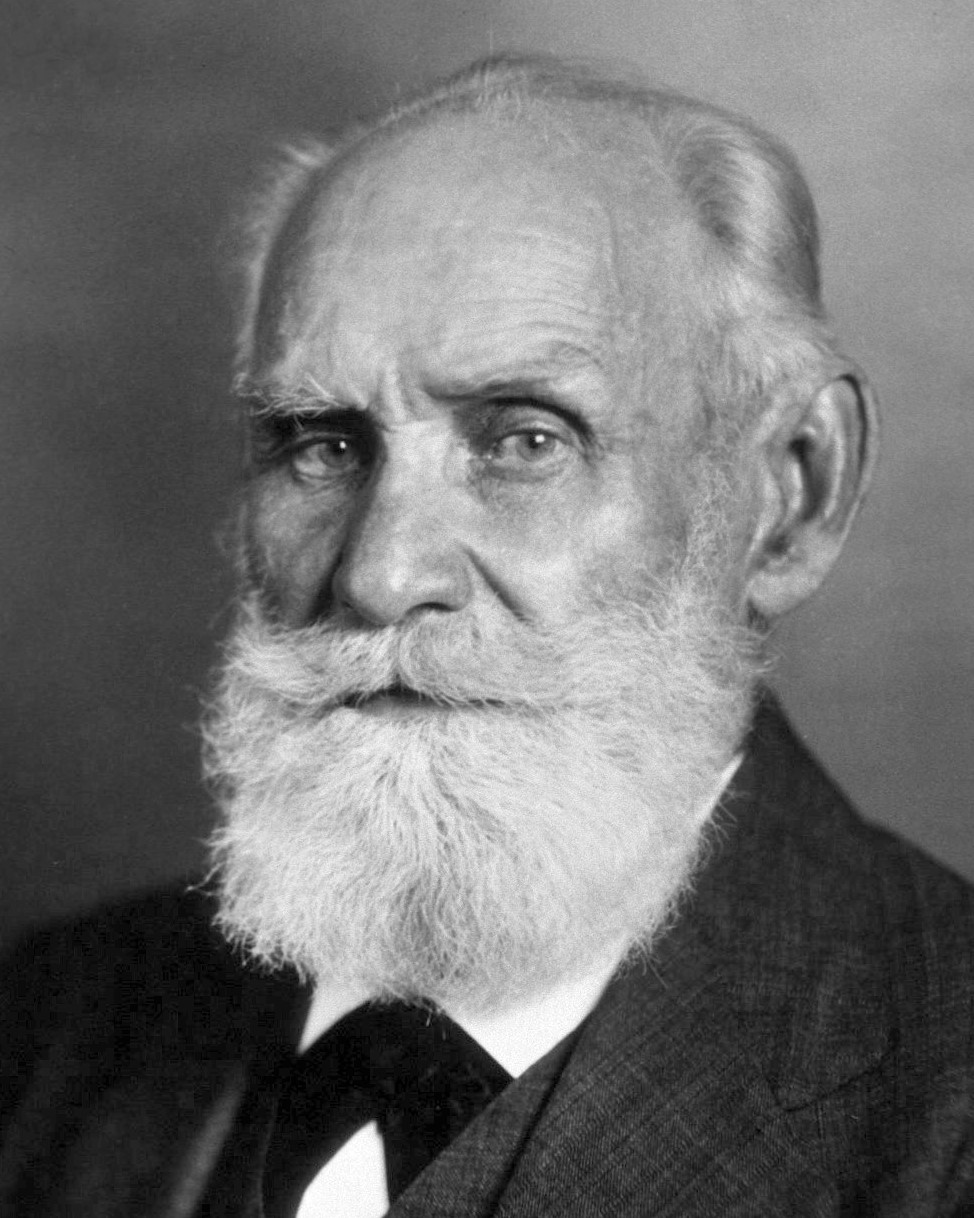
\includegraphics[width=3.0cm]{fig/lec01/Pavlov.jpg}
		\caption{Ivan Pavlov\\(1849-1936)}
	\end{figure}\vspace{-0.5cm}
	\begin{itemize}
		\item Classical conditioning
	\end{itemize}
\end{minipage}
\hfill
\begin{minipage}[t]{0.27\linewidth}
	\begin{figure}
		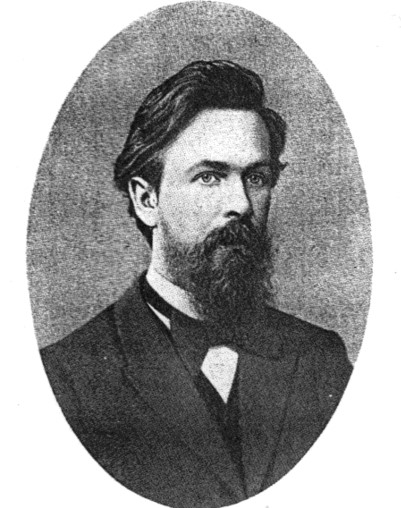
\includegraphics[width=3.0cm]{fig/lec01/Markov.jpg}
		\caption{Andrei Markov\\(1856-1922)}
	\end{figure}\vspace{-0.5cm}
	\begin{itemize}
		\item Stochastic process formalism 
	\end{itemize}
\end{minipage}
\hfill
\begin{minipage}[t]{0.27\linewidth}
	\begin{figure}
		
\includegraphics[width=3.0cm]{fig/lec01/Bell_man.pdf}
		\caption{Richard Bellman\\(1920-1984)\footnotemark}
	\end{figure}\vspace{-0.5cm}
	\begin{itemize}
		\item Optimal sequential decision making
	\end{itemize}
\end{minipage}
\footnotetext{Illustrative picture since an actual photo of Bellman is not freely available.}
}

%%%%%%%%%%%%%%%%%%%%%%%%%%%%%%%%%%%%%%%%%%%%%%%%%%%%%%%%%%%%%
%% RL History %%
%%%%%%%%%%%%%%%%%%%%%%%%%%%%%%%%%%%%%%%%%%%%%%%%%%%%%%%%%%%%%
\frame{\frametitle{History of reinforcement learning}
Huge field with many interconnections to different fields. One could give a lecture only on the historic development. Hence, interested readers are referred to:
\begin{itemize}
	\item Chapter 1.7 of Barto/Sutton, \textit{Reinforcement learning: an introduction}, 2nd edition, MIT Press, 2018 
	\item 30 minutes talk of A. Barto \href{https://www.youtube.com/watch?v=ul6B2oFPNDM}{(YouTube link)}
	\item Survey papers on historic as well as more recent developments: 
	\begin{itemize}
		\item Kaelbling et al., \textit{Reinforcement learning: A survey}, in Journal of Artificial Intelligence Research, vol. 4, pp. 237 - 285, 1996
		\item Arulkumaran et al., \textit{Deep reinforcement learning: a brief survey}, in IEEE Signal Processing Magazine, vol. 34, no. 6, pp. 26-38, 2017
		\item Botvinick et al., \textit{Reinforcement learning, fast and slow}, in Trends in Cognitive Sciences, vol. 23, iss. 5, pp. 408-422, 2019
	\end{itemize} 
\end{itemize}
}


%%%%%%%%%%%%%%%%%%%%%%%%%%%%%%%%%%%%%%%%%%%%%%%%%%%%%%%%%%%%%
%% Application Examples %%
%%%%%%%%%%%%%%%%%%%%%%%%%%%%%%%%%%%%%%%%%%%%%%%%%%%%%%%%%%%%%
\frame{\frametitle{Contemporary application examples}
Limited selection from a broad field:
\begin{itemize}
	\item \href{https://www.youtube.com/watch?v=hQ49Mc6LV78}{Controlling electric drive systems}
	\item \href{https://www.youtube.com/watch?v=Lt-KLtkDlh8}{Swinging-up and balance a cart-pole / an inverted pendulum}
	\item \href{https://www.youtube.com/watch?v=W_gxLKSsSIE}{Flipping pancakes with a roboter arm}
	\item \href{https://www.youtube.com/watch?v=opsmd5yuBF0}{Drifting with a RC-car}
	\item \href{https://www.youtube.com/watch?v=eRwTbRtnT1I}{Driving an autonomous car}
	\item \href{https://www.youtube.com/watch?v=eG1Ed8PTJ18}{Playing Atari Breakout}
	\item \href{https://www.youtube.com/watch?v=9xlSy9F5WtE}{Play strategy board game Go at super-human performance}
	\item \href{https://www.youtube.com/watch?v=kvblookYjA8}{Nuclear fusion reactor plasma control}
	\item \href{https://www.youtube.com/watch?v=VPRSBzXzavo}{Training chat bots (like chatGPT)}
	\item ...
\end{itemize}
}


%%%%%%%%%%%%%%%%%%%%%%%%%%%%%%%%%%%%%%%%%%%%%%%%%%%%%%%%%%%%%%%%%%
\section{Basic terminology} 
%%%%%%%%%%%%%%%%%%%%%%%%%%%%%%%%%%%%%%%%%%%%%%%%%%%%%%%%%%%%%%%%%%
\begin{frame}
\frametitle{Table of contents}
\tableofcontents[currentsection]
\end{frame}

%%%%%%%%%%%%%%%%%%%%%%%%%%%%%%%%%%%%%%%%%%%%%%%%%%%%%%%%%%%%%
%% Reward basics %%
%%%%%%%%%%%%%%%%%%%%%%%%%%%%%%%%%%%%%%%%%%%%%%%%%%%%%%%%%%%%%
\frame{\frametitle{Reward}
\begin{itemize}
	\item A \hl{reward} is a scalar \hl{random variable} $R_k$ with \hl{realizations} $r_k$.
	\item Often it is considered a real-number $r_k\in\mathbb{R}$ or an integer $r_k\in\mathbb{Z}$.\pause
	\item The reward function (interpreter) may be naturally given or is a design degree of freedom (i.e., can be manipulated).\pause 
	\item It fully indicates how well an RL agent is doing at step $k$.
	\item The agent's task is to \hl{maximize its reward over time}.\pause
\end{itemize}
\begin{theo}{Reward hypothesis}{reward_hypo}
All goals can be described by the maximization of the expected cumulative reward:
\begin{equation}
	\max \E{\sum_{i=0}^\infty R_{k+i+1}} .
\end{equation}
\end{theo} 
}


%%%%%%%%%%%%%%%%%%%%%%%%%%%%%%%%%%%%%%%%%%%%%%%%%%%%%%%%%%%%%
%% Reward examples %%
%%%%%%%%%%%%%%%%%%%%%%%%%%%%%%%%%%%%%%%%%%%%%%%%%%%%%%%%%%%%%
\frame{\frametitle{Reward examples}
\begin{itemize}
	\item Flipping a pancake:
	\begin{itemize}
		\item Pos. reward: catching the $\unit{180}{^\circ}$ rotated pancake 
		\item Neg. reward: droping the pancake on the floor
	\end{itemize}
	\pause
	\item Stock trading:
	\begin{itemize}
		\item Trading portfolio monetary value 
	\end{itemize}
	\pause
	\item Playing Atari games:
	\begin{itemize}
		\item Highscore value at the end of a game episode
	\end{itemize}
	\pause
	\item Driving an autonomous car:
	\begin{itemize}
		\item Pos. reward: getting save from A to B without crashing
		\item Neg. reward: hitting another car,  pedestrian, bicycle,...
	\end{itemize}
	\pause
	\item Classical control task (e.g., electric drive, inverted pendulum,...):
	\begin{itemize}
		\item Pos. reward: following a given reference trajectory precisely
		\item Neg. reward: violating system constraints and/or large control error
	\end{itemize}
\end{itemize}
}

%%%%%%%%%%%%%%%%%%%%%%%%%%%%%%%%%%%%%%%%%%%%%%%%%%%%%%%%%%%%%
%% Reward characteristics %%
%%%%%%%%%%%%%%%%%%%%%%%%%%%%%%%%%%%%%%%%%%%%%%%%%%%%%%%%%%%%%
\frame{\frametitle{Reward characteristics}
Rewards can have many different flavors and are highly depending on the given problem:
\begin{itemize}
	\item Actions may have short and/or long term consequences.
	\begin{itemize}
		\item The reward for a certain action may be delayed.
		\item Examples: Stock trading, strategic board games,...
	\end{itemize}
	\pause
	\item Rewards can be positive and negative real values.
	\begin{itemize}
		\item Certain situations (e.g. car hits wall) might lead to a negative reward.
	\end{itemize}
	\pause
	\item Exogenous impacts might introduce stochastic reward components.
\begin{itemize}
	\item Example: A wind gust pushes the helicopter into a tree. 
\end{itemize}
\end{itemize}
\pause
\begin{block}{Remark on reward}
The RL agent's learning process is heavily linked with the reward distribution over time. Designing expedient rewards functions is therefore crucially important for successfully applying RL. And often there is no predefined way on how to design the ``best reward function''.
\end{block}
}

%%%%%%%%%%%%%%%%%%%%%%%%%%%%%%%%%%%%%%%%%%%%%%%%%%%%%%%%%%%%%
%% King Midas %%
%%%%%%%%%%%%%%%%%%%%%%%%%%%%%%%%%%%%%%%%%%%%%%%%%%%%%%%%%%%%%
\frame{\frametitle{The reward function hassle}
\begin{itemize}
	\item ``Be careful what you wish for - you might get it'' (pro-verb)
	\item ``...it grants what you ask for, not what you should have asked for or what you intend.'' (Norbert Wiener, American mathematician)
\end{itemize}
\begin{figure}
		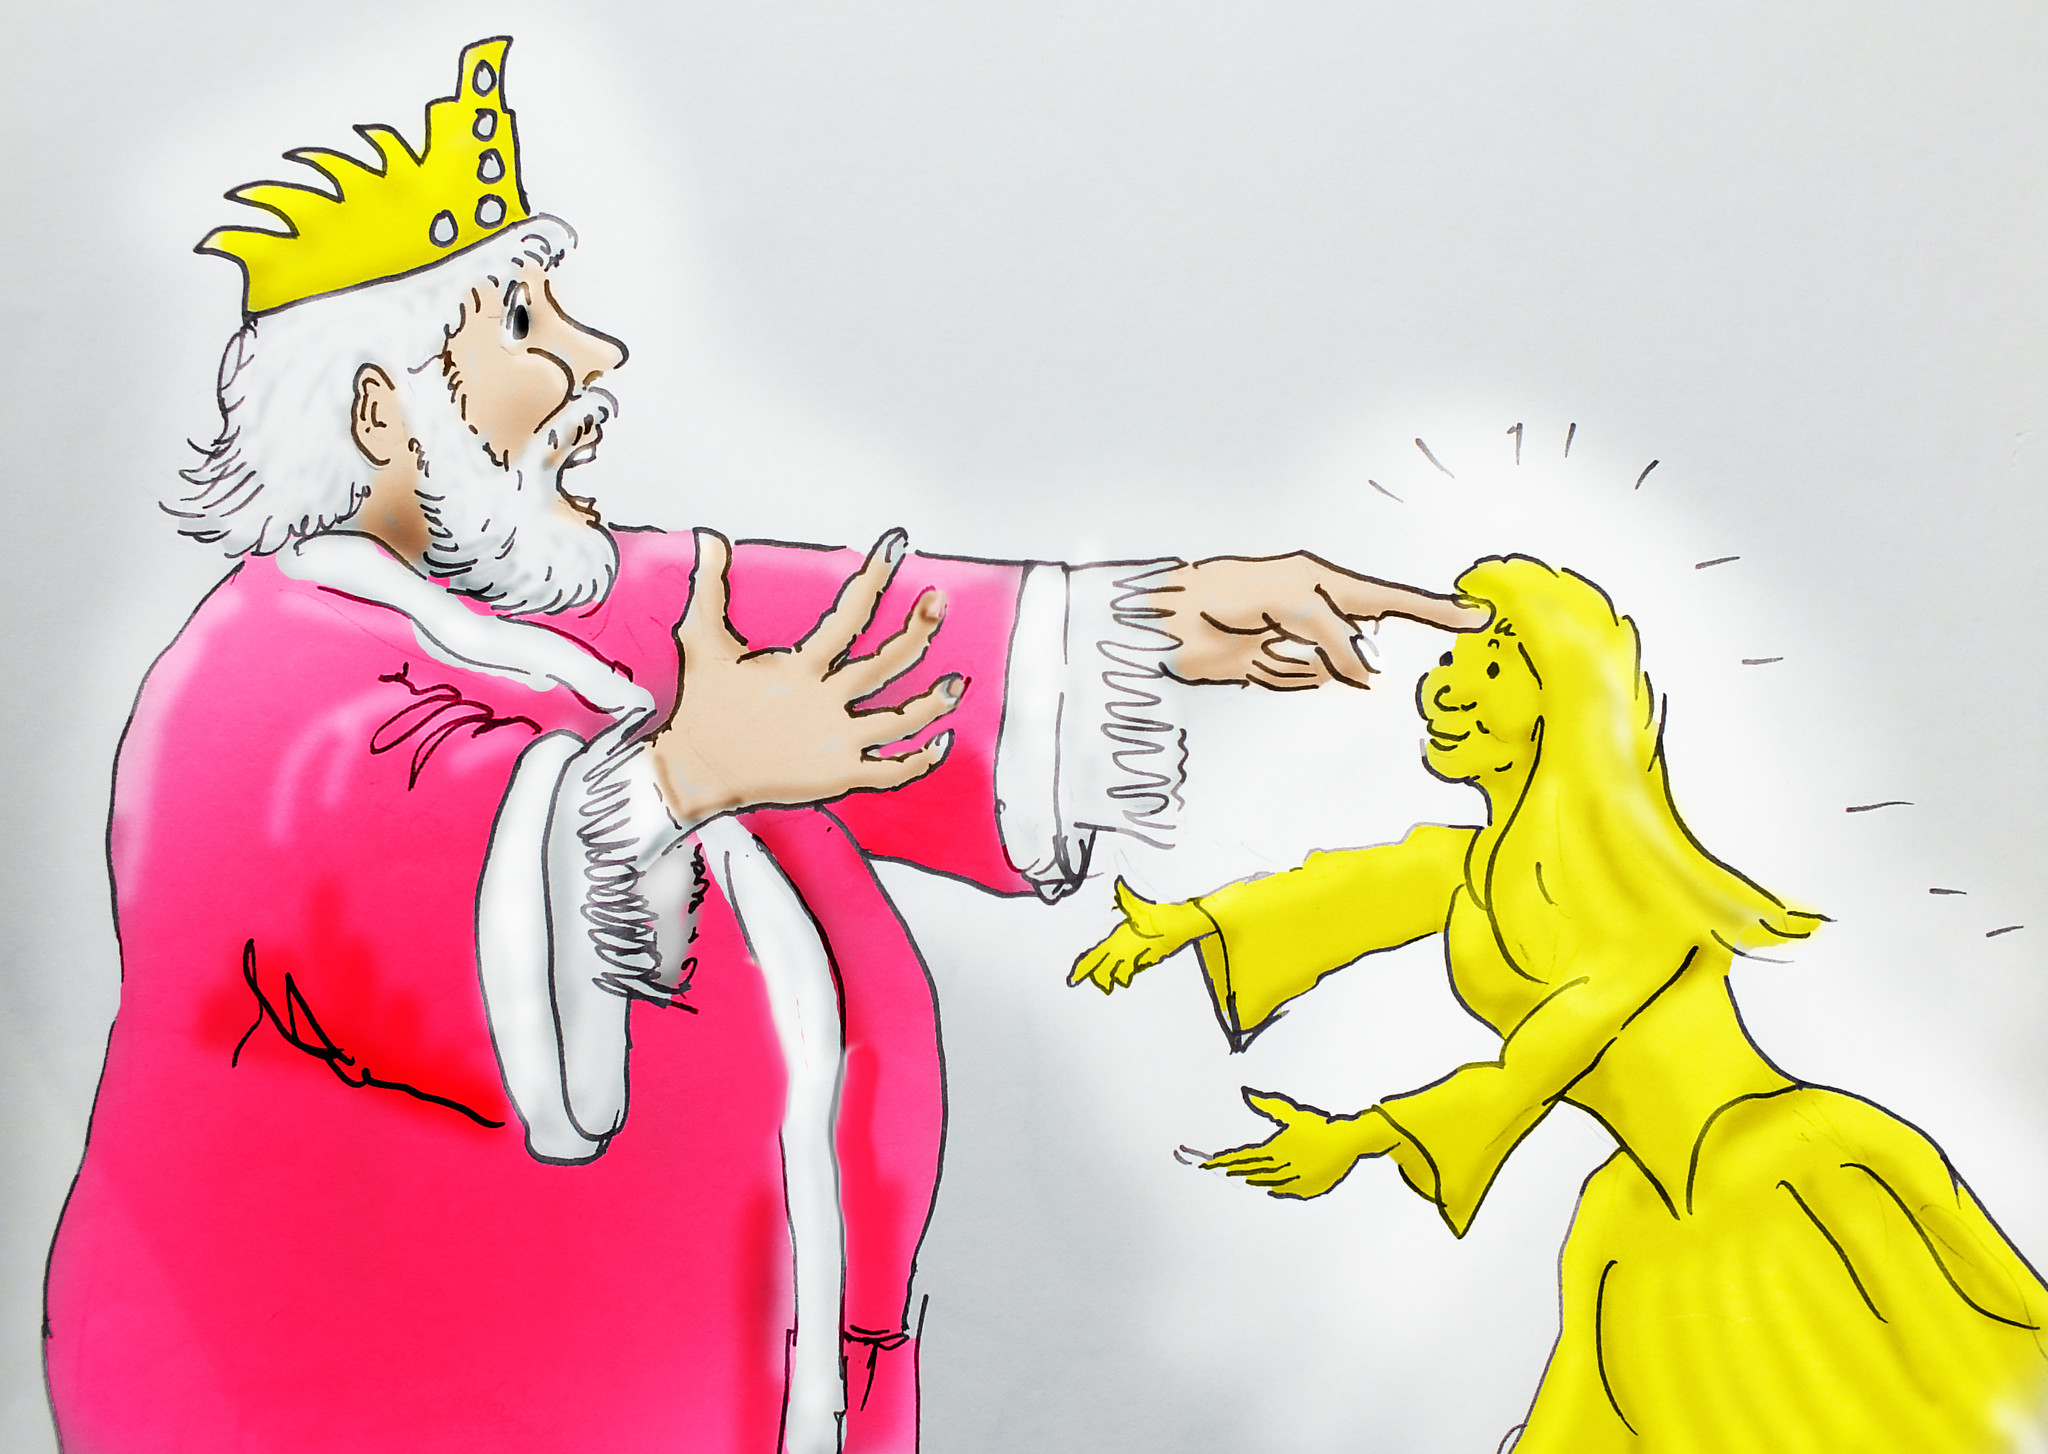
\includegraphics[width=6cm]{fig/lec01/Midas.jpg}
		\caption{Midas and daughter (good as gold)\\(source: \href{https://www.flickr.com/photos/robinhutton/16403846414/in/photostream/}{www.flickr.com}, by \href{https://www.flickr.com/photos/robinhutton/}{Robin Hutton} \href{https://creativecommons.org/licenses/by-nc-nd/2.0/}{CC BY-NC-ND 2.0})}
		\label{fig:Midas}
	\end{figure}
}

%%%%%%%%%%%%%%%%%%%%%%%%%%%%%%%%%%%%%%%%%%%%%%%%%%%%%%%%%%%%%
%% Task-dependent return definitions %%
%%%%%%%%%%%%%%%%%%%%%%%%%%%%%%%%%%%%%%%%%%%%%%%%%%%%%%%%%%%%%
\frame{\frametitle{Task-dependent return definitions}
\hlh{Episodic tasks}
\begin{itemize}
	\item A problem which naturally breaks into subsequences (\hl{finite horizon}).
	\item Examples: most games, maze,...
	\item The \hl{return} becomes a finite sum:
	\begin{equation}
	g_k = r_{k+1} + r_{k+2} + \cdots + r_{N}\, .	
	\end{equation}
	\item Episodes end at their terminal step $k=N$.
\end{itemize}
\pause
\hlh{Continuing tasks}
\begin{itemize}
	\item A problem which lacks a natural end (\hl{infinite horizon}).
	\item Example: process control task
	\item The return should be \hl{discounted} to prevent infinite numbers:
	\begin{equation}
	\label{eq:return_disc}
	g_k = r_{k+1} + \gamma r_{k+2} + \gamma^2 r_{k+3} + \cdots = \sum_{i=0}^\infty \gamma^i r_{k+i+1}\, .  	
	\end{equation}
	\item Here, $\gamma\in\left\{\mathbb{R}|0 \leq \gamma \leq 1\right\}$ is the \hl{discount rate}.
\end{itemize}
}

%%%%%%%%%%%%%%%%%%%%%%%%%%%%%%%%%%%%%%%%%%%%%%%%%%%%%%%%%%%%%
%% Disounted rewards %%
%%%%%%%%%%%%%%%%%%%%%%%%%%%%%%%%%%%%%%%%%%%%%%%%%%%%%%%%%%%%%
\frame{\frametitle{Discounted rewards}
\hlh{Numeric viewpoint}
\begin{itemize}
	\item If $\gamma =1$ and $r_k > 0$ for $k\rightarrow\infty$, $g_k$ in \eqref{eq:return_disc} gets infinite.
	\item If $\gamma <1$ and $r_k$ is bounded for $k\rightarrow\infty$, $g_k$ in \eqref{eq:return_disc} is bounded.
\end{itemize}
\pause
\hlh{Strategic viewpoint}
\begin{itemize}
	\item If $\gamma \approx 1$: agent is farsighted.
	\item If $\gamma \approx 0$: agent is shortsighted (only interested in immediate reward).
\end{itemize}
\pause
\hlh{Mathematical options}
\begin{itemize}
	\item The current return is the discounted future return:
\begin{equation}
	\begin{split}
		g_k &= r_{k+1} + \gamma r_{k+2} + \gamma^2 r_{k+3} + \cdots = r_{k+1} + \gamma \left(r_{k+2} + \gamma r_{k+3} + \cdots \right)\\
				&= r_{k+1} + \gamma g_{k+1}\, .
	\end{split}
\end{equation}
\pause
	\item If $r_k=r$ is a constant and $\gamma<1$ one receives:
	\begin{equation}
		g_k = \sum_{i=0}^\infty \gamma^i r = r \sum_{i=0}^\infty \gamma^i = r\frac{1}{1-\gamma}\, .
	\end{equation}
\end{itemize}
}

%%%%%%%%%%%%%%%%%%%%%%%%%%%%%%%%%%%%%%%%%%%%%%%%%%%%%%%%%%%%%
%% The env. state %%
%%%%%%%%%%%%%%%%%%%%%%%%%%%%%%%%%%%%%%%%%%%%%%%%%%%%%%%%%%%%%
\frame{\frametitle{State (1)}
\hlh{Environment state}  \blfootnote{\hl{Bold symbols} are non-scalar multidimensional quantities, e.g., vectors and matrices.}
\begin{itemize}
	\item Random variable $\bm{X}_k^e$ with realizations $\bm{x}_k^e$ \blfootnote{\hl{Capital symbols} denote random variables and small symbols their realizations.}
	\item Internal status representation of the environment, e.g.,
	\begin{itemize}
		\item Physical states, e.g., car velocity or motor current
		\item Game states, e.g., current chess board situation
		\item Financial states, e.g., stock market status 
	\end{itemize}
	\pause
	\item  Fully, limited or not at all visible by the agent
	\begin{itemize}
		\item Sometimes even 'foggy' or uncertain
		\item In general: $\bm{Y}_k = \bm{f}(\bm{X}_k)$ as the measurable outputs of the environment
	\end{itemize}
	\pause
	\item Continuous or discrete quantity
\end{itemize}
}

%%%%%%%%%%%%%%%%%%%%%%%%%%%%%%%%%%%%%%%%%%%%%%%%%%%%%%%%%%%%%
%% The act. state %%
%%%%%%%%%%%%%%%%%%%%%%%%%%%%%%%%%%%%%%%%%%%%%%%%%%%%%%%%%%%%%
\frame{\frametitle{State (2)}
\hlh{Agent state} 
\begin{itemize}
  \item Random variable $\bm{X}_k^a$ with realizations $\bm{x}_k^a$ 
	\item Internal status representation of the agent
	\pause
	\item In general: $\bm{x}_k^a\neq \bm{x}_k^e$, e.g., due to measurement noise or an additional agent's memory
	\pause
	\item Agent's condensed information relevant for next action
	\item Dependent on internal knowledge / policy representation of the agent
	\pause
	\item Continuous or discrete quantity
\end{itemize}
}

%%%%%%%%%%%%%%%%%%%%%%%%%%%%%%%%%%%%%%%%%%%%%%%%%%%%%%%%%%%%%
%% History and Imformation State%%
%%%%%%%%%%%%%%%%%%%%%%%%%%%%%%%%%%%%%%%%%%%%%%%%%%%%%%%%%%%%%
\frame{\frametitle{History and information state}
\begin{defi}{History}{History}
The history is the past sequence of all observations, actions and rewards
\begin{equation}
	\mathbb{H}_k = \left\{\bm{y}_0, r_0, \bm{u}_0, \ldots, \bm{u}_{k-1}, \bm{y}_k, r_k\right\}
\end{equation}
up to the time step $k$.
\end{defi}
\pause
If the current state $\bm{x}_k$ contains all useful information from the history it is called an \hl{information or Markov state} (history is fully condensed in $\bm{x}_k$):
\begin{defi}{Information state}{InfSate}
A state $\bm{X}_k$ is called an information state if and only if
\begin{equation}
	\Pb{\bm{X}_{k+1}|\bm{X}_k}=\Pb{\bm{X}_{k+1}|\bm{X}_0, \bm{X}_1,\ldots, \bm{X}_k}\, .
\end{equation}
\end{defi}
}

%%%%%%%%%%%%%%%%%%%%%%%%%%%%%%%%%%%%%%%%%%%%%%%%%%%%%%%%%%%%%
%% State Example%%
%%%%%%%%%%%%%%%%%%%%%%%%%%%%%%%%%%%%%%%%%%%%%%%%%%%%%%%%%%%%%
\frame{\frametitle{Model examples with Markov states}
Linear time-invariant (LTI) state-space model
\begin{equation}
\begin{split}
	\bm{x}_{k+1} &= \bm{A}\bm{x}_k +\bm{B}\bm{u}_k\, ,\\
	\bm{y}_{k} &= \bm{C}\bm{x}_k+ \bm{D}\bm{u}_k\, .
\end{split}
\end{equation}
\pause
\vspace{0.5cm}

Nonlinear time-invariant state-space model:
\begin{equation}
\begin{split}
	\bm{x}_{k+1} &= \bm{f}\left(\bm{x}_k, \bm{u}_k\right)\, ,\\
	\bm{y}_{k} &= \bm{h}\left(\bm{x}_k, \bm{u}_k\right)\,.
\end{split}
\end{equation}
}

%%%%%%%%%%%%%%%%%%%%%%%%%%%%%%%%%%%%%%%%%%%%%%%%%%%%%%%%%%%%%
%% State Example%%
%%%%%%%%%%%%%%%%%%%%%%%%%%%%%%%%%%%%%%%%%%%%%%%%%%%%%%%%%%%%%
\frame{\frametitle{Degree of observability}

\hlh{Full observability}
	\begin{itemize}
		\item Agent directly measures full environment state (e.g., $\bm{y}_k = \bm{I}\bm{x}_k$).
		\item If $\bm{x}_k$ is Markov: Markov decision process (MDP).
	\end{itemize}
\vspace{0.5cm}
\pause
\hlh{Partial observability}
	\begin{itemize}
		\item Agent does not have full access to environment state (e.g., $\bm{y}_k = \begin{bmatrix}\bm{I} & 0 \\ 0 & 0\end{bmatrix}\bm{x}_k$).
		\item If $\bm{x}_k$ is Markov: partial observable MDP (POMDP).
		\item Agent may reconstructs state information $\hat{\bm{x}}_k\approx \bm{x}_k$ (belief, estimate).
	\end{itemize}
\vspace{0.5cm}
\pause
\hlh{POMDP examples}
	\begin{itemize}
	\item Technical systems with limited sensors (cutting costs)
	\item Poker game (unknown opponents' cards)
	\item Human health status (too complex system)
\end{itemize}
}

%%%%%%%%%%%%%%%%%%%%%%%%%%%%%%%%%%%%%%%%%%%%%%%%%%%%%%%%%%%%%
%% Actions%%
%%%%%%%%%%%%%%%%%%%%%%%%%%%%%%%%%%%%%%%%%%%%%%%%%%%%%%%%%%%%%
\frame{\frametitle{Action}
\begin{itemize}
	\item An \hl{action} is the agent's degree of freedom in order to maximize its reward.
	\pause
	\item Major distinction:
	\begin{itemize}
		\item \hl{Finite action set} (FAS): $\bm{u}_k\in\left\{\bm{u}_{k,1},\bm{u}_{k,2},\ldots\right\}\in\mathbb{R}^m$
		\item \hl{Continuous action set} (CAS): Infinite number of actions: $\bm{u}_k\in\mathbb{R}^m$
		\item Deterministic $\bm{u}_k$ or random $\bm{U}_k$ variable
		\item Often state-dependent and potentially constrained:$\bm{u}_k\in\mathcal{U}(\bm{x}_k)\subseteq\mathbb{R}^m$  \pause
	\end{itemize}
	\item Examples:
	\begin{itemize}
		\item Take a card during Black Jack game (FAS) \pause
				\item Drive an autonomous car (CAS) \pause
		\item Buy stock options for your trading portfolio (FAS/CAS) \pause
	\end{itemize}
\end{itemize}
\begin{block}{Remark on state and action spaces}
Evaluating the state and action spaces (e.g., finite vs. continuous) of a new RL problem should be always the first steps in order to choose appropriate solution algorithms.  
\end{block}
}

%%%%%%%%%%%%%%%%%%%%%%%%%%%%%%%%%%%%%%%%%%%%%%%%%%%%%%%%%%%%%
%% Actions%%
%%%%%%%%%%%%%%%%%%%%%%%%%%%%%%%%%%%%%%%%%%%%%%%%%%%%%%%%%%%%%
\frame{\frametitle{Policy}
\begin{itemize}
\item A \hl{policy} $\bm{\pi}$ is the agent's internal strategy on picking actions.\pause
\item Deterministic policies:  maps state and action directly:
\begin{equation}
	\bm{u}_k = \bm{\pi}(\bm{x}_k)\, .
\end{equation}
\pause
\item Stochastic policies: maps a probability of the action given a state:
\begin{equation}
	\bm{\pi}(\bm{U}_k|\bm{X}_k)=\Pb{\bm{U}_k | \bm{X}_k}\, .
\end{equation}
\pause
\item RL is all about changing $\bm{\pi}$ over time in order to maximize the expected return.
\end{itemize}
}

%%%%%%%%%%%%%%%%%%%%%%%%%%%%%%%%%%%%%%%%%%%%%%%%%%%%%%%%%%%%%
%% Deterministic policy example %%
%%%%%%%%%%%%%%%%%%%%%%%%%%%%%%%%%%%%%%%%%%%%%%%%%%%%%%%%%%%%%
\frame{\frametitle{Deterministic policy example}
\onslide<1->Find optimal gains $\{K_\mathrm{p}, K_\mathrm{i}, K_\mathrm{d}\}$ given the reward $r_k=-e_k^2$:
\begin{itemize}
	\onslide<2->\item Agent's behavior is explicitly determined by $\{K_\mathrm{p}, K_\mathrm{i}, K_\mathrm{d}\}$.
	\onslide<3->\item	Reference value is part of the environment state: $\bm{x}_k = \begin{bmatrix}y_k & y^*_k\end{bmatrix}\T$.
	\onslide<4->\item Control output is the agent's action: $\bm{u}_k = \bm{\pi}(\bm{x}_k|K_\mathrm{p}, K_\mathrm{i}, K_\mathrm{d})$.
\end{itemize}

\onslide<1->\begin{figure}
	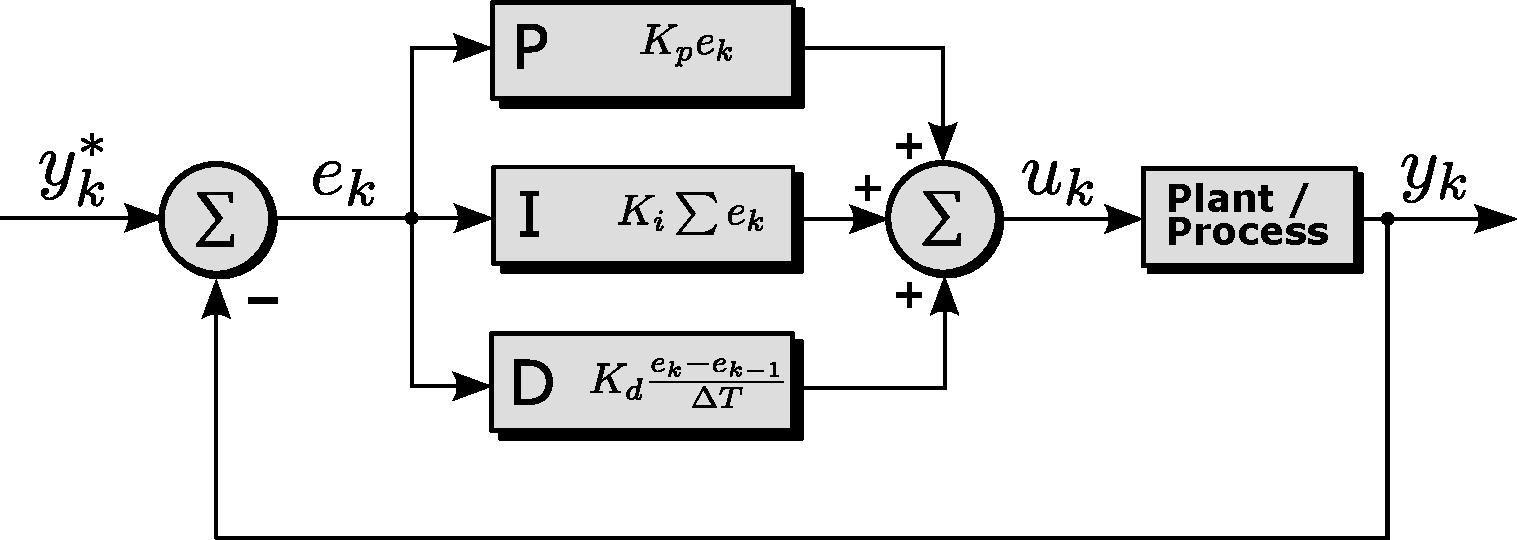
\includegraphics[width=10cm]{fig/lec01/Control_Loop.pdf}
	\caption{Classical PID control loop with scalar quantities (derivative of \href{https://en.wikipedia.org/wiki/PID_controller}{www.wikipedia.org}, by Arturo Urquizo \href{https://creativecommons.org/licenses/by-sa/3.0/deed.en}{CC BY-SA 3.0})}
	\label{fig:Control_Loop_PID}
\end{figure}
}

%%%%%%%%%%%%%%%%%%%%%%%%%%%%%%%%%%%%%%%%%%%%%%%%%%%%%%%%%%%%%
%% Stochastic policy example %%
%%%%%%%%%%%%%%%%%%%%%%%%%%%%%%%%%%%%%%%%%%%%%%%%%%%%%%%%%%%%%
\frame{\frametitle{Stochastic policy example}
\onslide<1->Two-player game of extended rock-paper-scissors: 
\begin{itemize}
	\onslide<2->\item A deterministic policy can be easily exploited by the opponent.
	\onslide<3->\item	A uniform random policy would be instead unpredictable (assuming an ideal random number generator).
\end{itemize}

\onslide<1->
\begin{figure}
	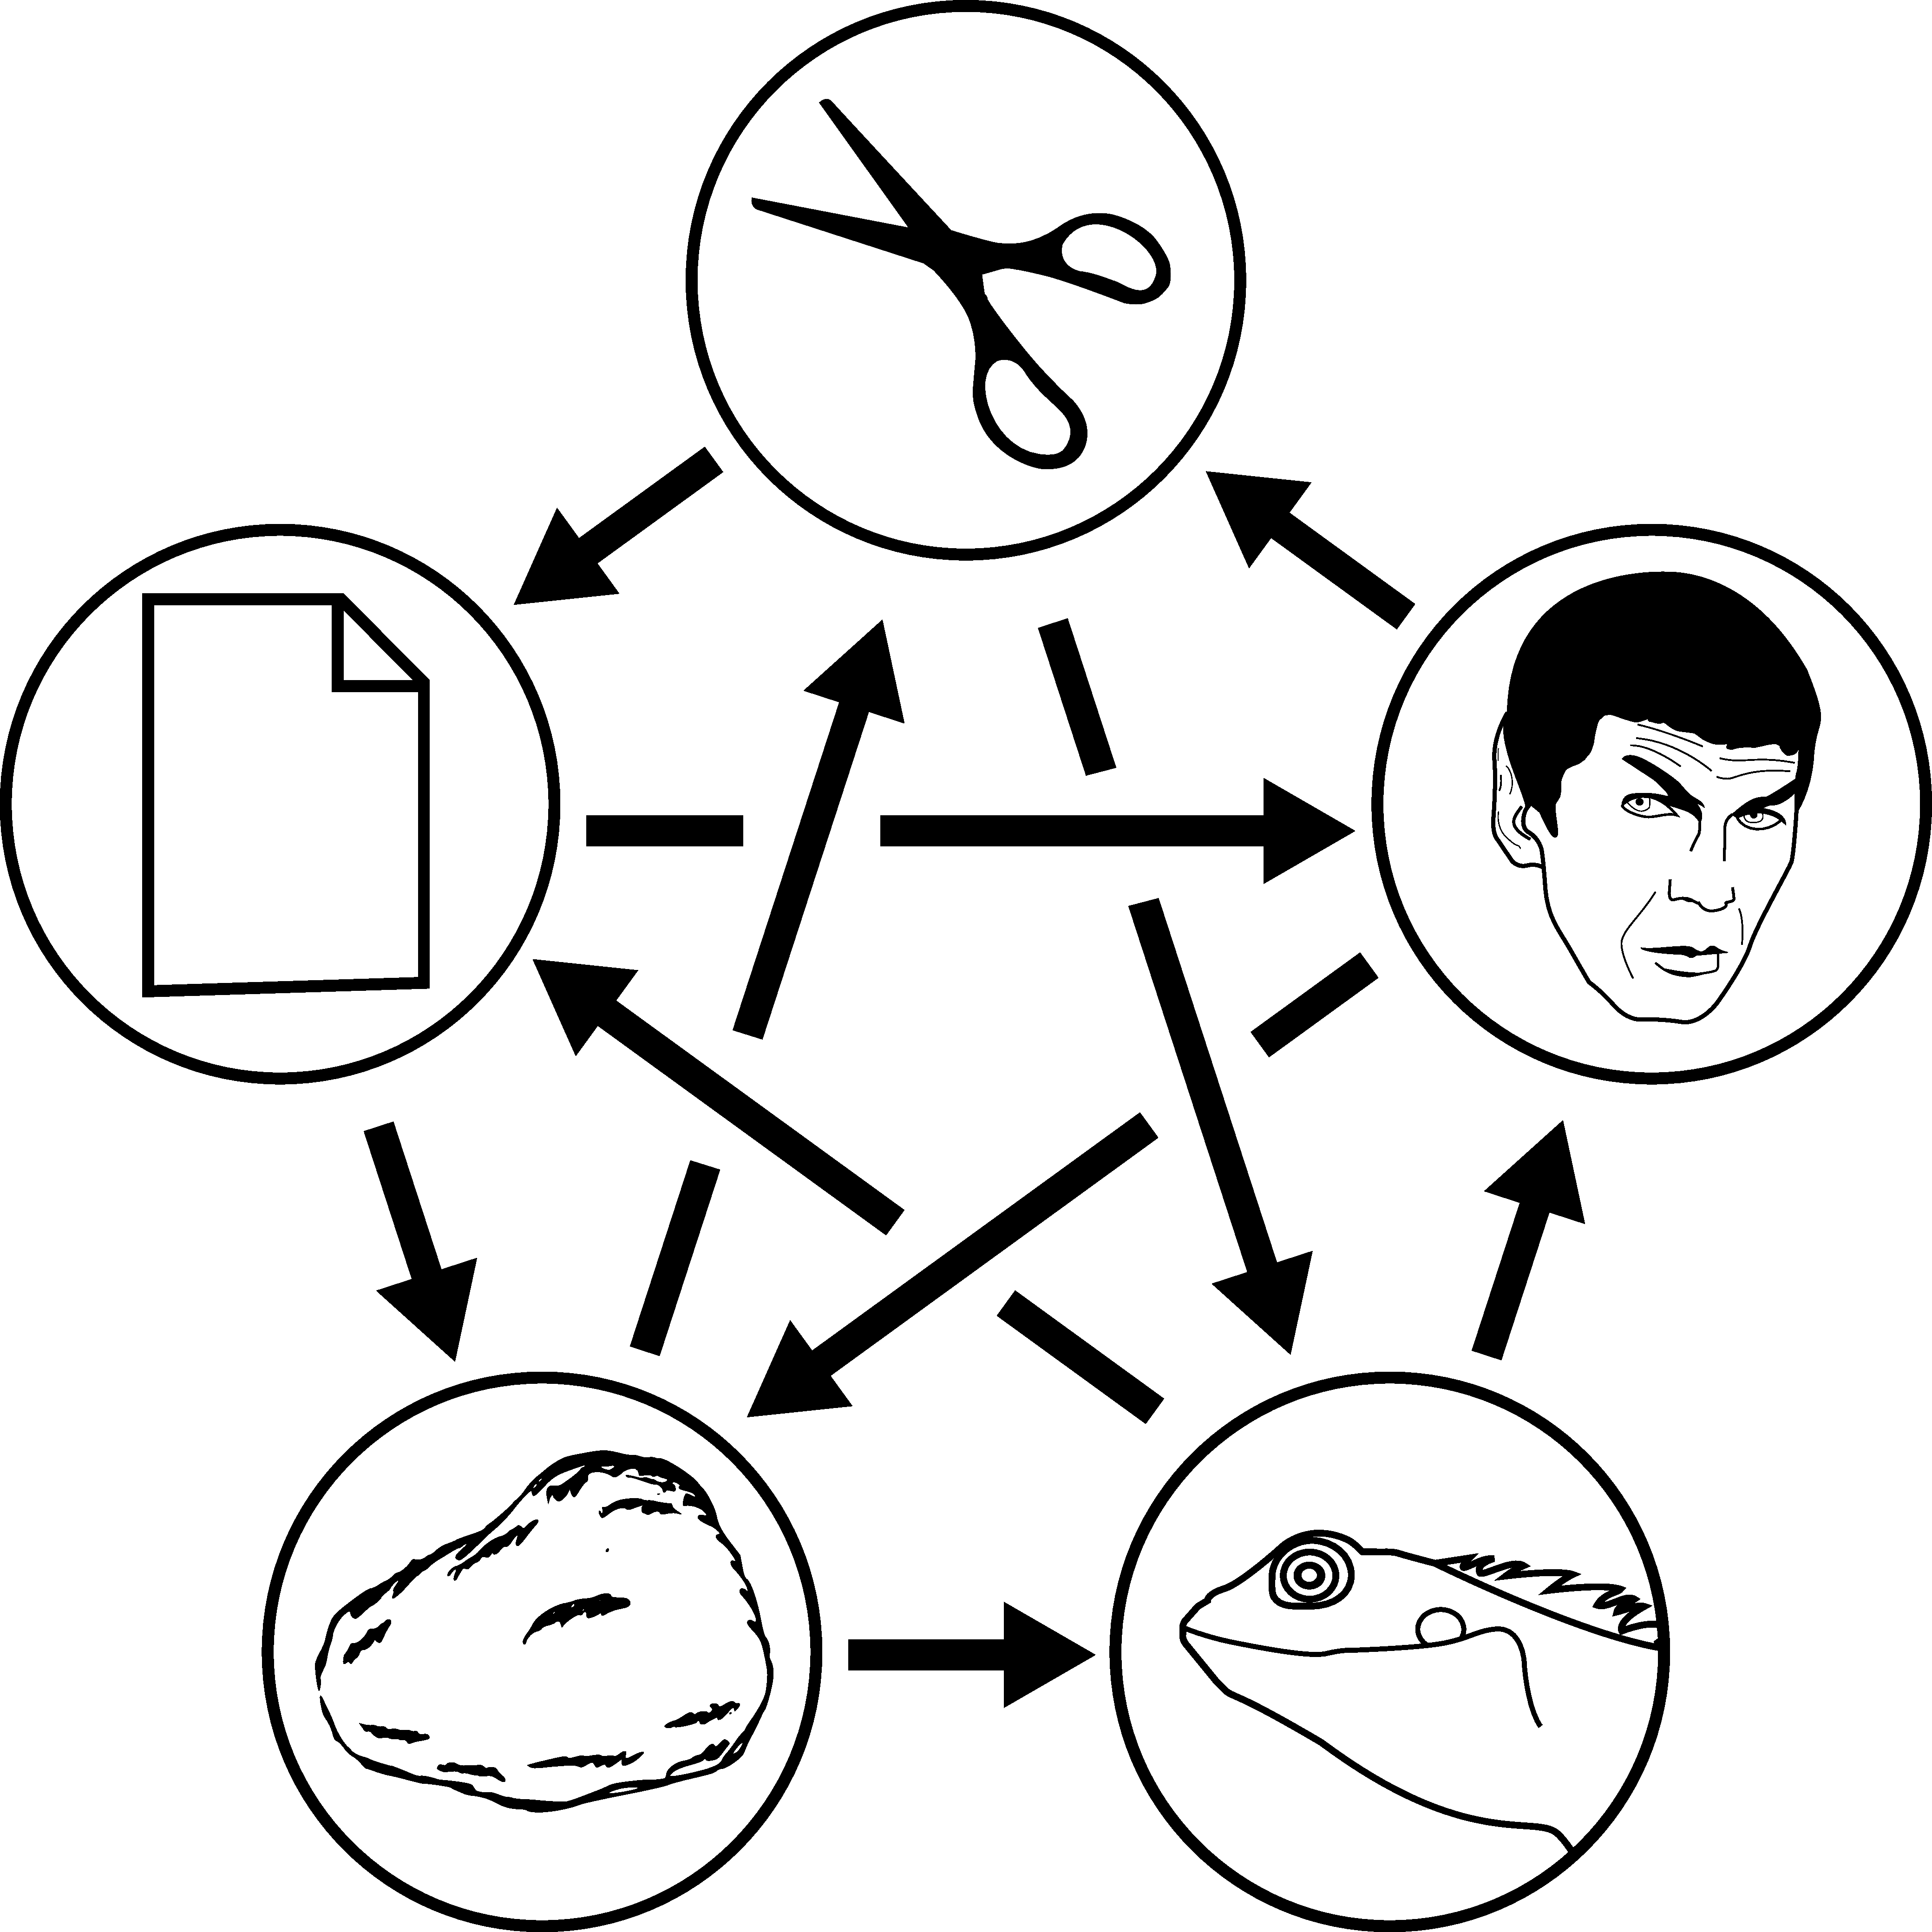
\includegraphics[height=0.45\textheight]{fig/lec01/Rock_paper_scissors_lizard_spock.pdf}
	\caption{Rock paper scissors lizard Spock game mechanics\\(source: \href{https://commons.wikimedia.org/wiki/File:Rock_paper_scissors_lizard_spock.svg}{www.wikipedia.org},  by \href{https://en.wikipedia.org/wiki/User:Diriector_Doc}{Diriector Doc} \href{https://creativecommons.org/licenses/by-sa/4.0/deed.en}{CC BY-SA 4.0})}
	\label{fig:Rock_paper_scissors_lizard_spock}
\end{figure}
}

%%%%%%%%%%%%%%%%%%%%%%%%%%%%%%%%%%%%%%%%%%%%%%%%%%%%%%%%%%%%%
%% Value function %%
%%%%%%%%%%%%%%%%%%%%%%%%%%%%%%%%%%%%%%%%%%%%%%%%%%%%%%%%%%%%%
\frame{\frametitle{Value functions}
\begin{itemize}
	\item The \hl{state-value function} is the expected return being in state $\bm{x}_k$ following a policy $\bm{\pi}$: $v_\pi(\bm{x}_k)$.
	\pause
	\item Assuming an MDP problem structure the state-value function is
	\begin{equation}
	\label{eq:state_value_lec01}
		v_\pi(\bm{x}_k) = \El{G_k|\bm{X}_k=\bm{x}_k}{\pi}=\El{\left. \sum_{i=0}^\infty \gamma^i R_{k+i+1}\right|\bm{x}_k}{\pi}.
	\end{equation}
	\pause
\item The \hl{action-value function} is the expected return being in state $\bm{x}_k$ taken an action $\bm{u}_k$ and, thereafter, following a policy $\bm{\pi}$: $q_\pi(\bm{x}_k, \bm{u}_k)$.
\pause
	\item Assuming an MDP problem structure the action-value function is
\end{itemize}
	\begin{equation}
		q_\pi(\bm{x}_k,\bm{u}_k) = \El{G_k|\bm{X}_k=\bm{x}_k, \bm{U}_k=\bm{u}_k}{\pi}=\El{\left.\sum_{i=0}^\infty \gamma^i R_{k+i+1}\right|\bm{x}_k, \bm{u}_k}{\pi}.
	\end{equation}\pause
\begin{itemize}
	\item A key task in RL is to estimate $v_\pi(\bm{x}_k)$ and $q_\pi(\bm{x}_k,\bm{u}_k)$ based on sampled data.
\end{itemize}
}

%%%%%%%%%%%%%%%%%%%%%%%%%%%%%%%%%%%%%%%%%%%%%%%%%%%%%%%%%%%%%
%% Model %%
%%%%%%%%%%%%%%%%%%%%%%%%%%%%%%%%%%%%%%%%%%%%%%%%%%%%%%%%%%%%%
\frame{\frametitle{Model}
\begin{itemize}
	\item A \hl{model} predicts what will happen inside an environment.\pause
	\item That could be a state model $\bm{\mathcal{P}}$:
	\begin{equation}
		\bm{\mathcal{P}} = \Pb{\bm{X}_{k+1}=\bm{x}_{k+1}|\bm{X}_k=\bm{x}_k, \bm{U}_k=\bm{u}_k}\,.
	\end{equation}
	\pause
	\item Or a reward model $\mathcal{R}$:
	\begin{equation}
		\mathcal{R} = \Pb{R_{k+1}=r_{k+1}|\bm{X}_k=\bm{x}_k, \bm{U}_k=\bm{u}_k}\,.
	\end{equation}
	\pause
	\item In general, those models could be stochastic (as denoted above) but in some problems relax to a deterministic form.\pause
	\item Using data in order to fit a model is a learning problem of its own and often called \hl{system identification}.
\end{itemize}
}

%%%%%%%%%%%%%%%%%%%%%%%%%%%%%%%%%%%%%%%%%%%%%%%%%%%%%%%%%%%%%
%% Exploration and Exploitation %%
%%%%%%%%%%%%%%%%%%%%%%%%%%%%%%%%%%%%%%%%%%%%%%%%%%%%%%%%%%%%%
\frame{\frametitle{Exploration and exploitation}
\begin{itemize}
	\item In RL the environment is initially unknown. How to act optimal?
	\item \hl{Exploration}: find out more about the environment.
	\item \hl{Exploitation}: maximize current reward using limited
	information.\pause
	\item Trade-off problem: what's the best split between both strategies?
\end{itemize}	
\begin{figure}
	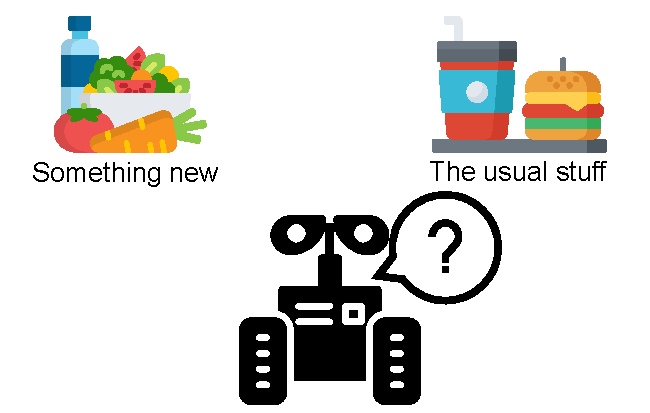
\includegraphics[width=7cm]{fig/lec01/Exploration_Exploitation.pdf}
	\caption{The exploration-exploitation dilemma}
	\label{fig:Exploration_Exploitation}
\end{figure}
}

%%%%%%%%%%%%%%%%%%%%%%%%%%%%%%%%%%%%%%%%%%%%%%%%%%%%%%%%%%%%%%%%%%
\section{Main categories of reinforcement learning algorithms} 
%%%%%%%%%%%%%%%%%%%%%%%%%%%%%%%%%%%%%%%%%%%%%%%%%%%%%%%%%%%%%%%%%%
\begin{frame}
\frametitle{Table of contents}
\tableofcontents[currentsection]
\end{frame}

%%%%%%%%%%%%%%%%%%%%%%%%%%%%%%%%%%%%%%%%%%%%%%%%%%%%%%%%%%%%%
%% Maze Example%%
%%%%%%%%%%%%%%%%%%%%%%%%%%%%%%%%%%%%%%%%%%%%%%%%%%%%%%%%%%%%%
\frame{\frametitle{Maze example}
\begin{minipage}[c]{0.5\linewidth}
	\begin{figure}
		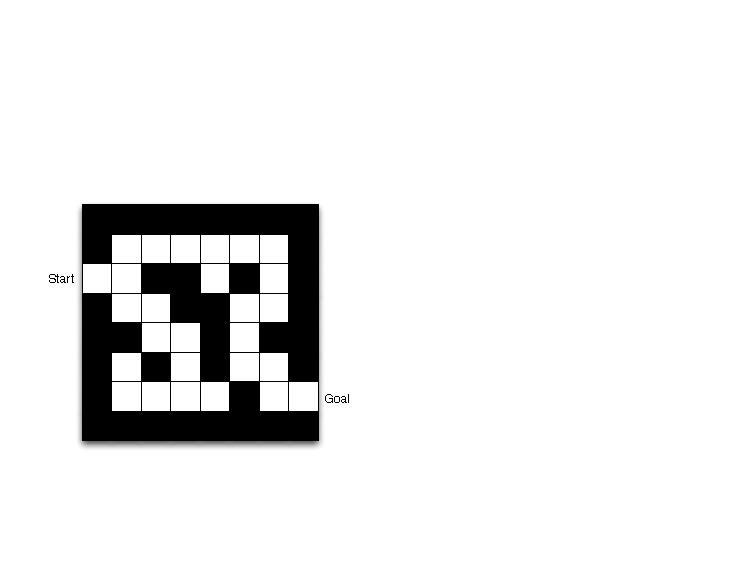
\includegraphics[width=6cm]{fig/lec01/Maze_Basic.pdf}
		\caption{Maze setup\\ \SilverLectureSource}
		\label{fig:Maze_Basic}
	\end{figure}
\end{minipage}
\hfill
\begin{minipage}[c]{0.47\linewidth}
\vspace{0.3cm}
Problem statement:
	\begin{itemize}
		\item Reward: $r_k=-1$ 
		\item At goal: episode termination
		\item Actions: $u_k\in\left\{N, E, S, W\right\}$
		\item State: agent's location
		\item Deterministic problem (no stochastic influences)
	\end{itemize}
\end{minipage}
}

%%%%%%%%%%%%%%%%%%%%%%%%%%%%%%%%%%%%%%%%%%%%%%%%%%%%%%%%%%%%%
%% Maze Policy%%
%%%%%%%%%%%%%%%%%%%%%%%%%%%%%%%%%%%%%%%%%%%%%%%%%%%%%%%%%%%%%
\frame{\frametitle{Maze example: RL-solution by policy}
\begin{minipage}[c]{0.55\linewidth}
	\begin{figure}
		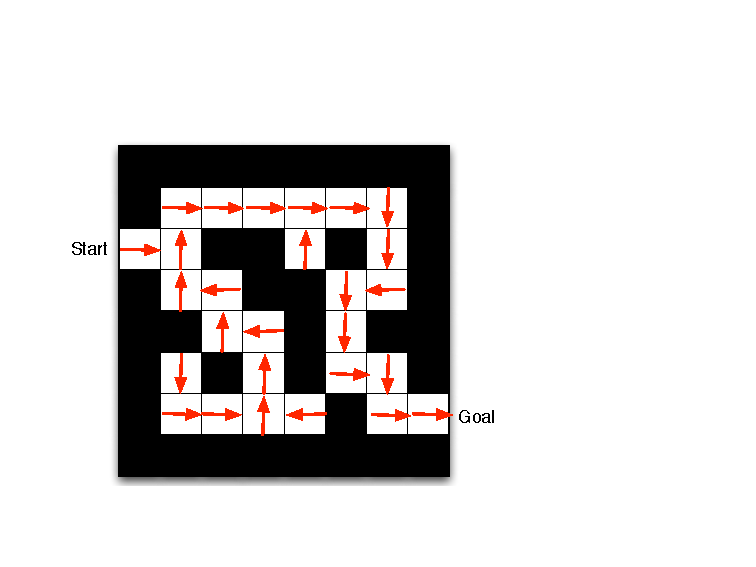
\includegraphics[width=6cm]{fig/lec01/Maze_Policy.pdf}
		\caption{Arrows represent policy $\pi(x_k)$ \SilverLectureSource}
		\label{fig:Maze_Policy}
	\end{figure}
\end{minipage}
\hfill
\begin{minipage}[c]{0.43\linewidth}
Key characteristics:
	\begin{itemize}
		\item For any state there is a direct action command.
		\item The policy is explicitly available.
	\end{itemize}
\end{minipage}
}

%%%%%%%%%%%%%%%%%%%%%%%%%%%%%%%%%%%%%%%%%%%%%%%%%%%%%%%%%%%%%
%% Maze Value%%
%%%%%%%%%%%%%%%%%%%%%%%%%%%%%%%%%%%%%%%%%%%%%%%%%%%%%%%%%%%%%
\frame{\frametitle{Maze example: RL-solution by value function}
\begin{minipage}[c]{0.55\linewidth}
	\begin{figure}
		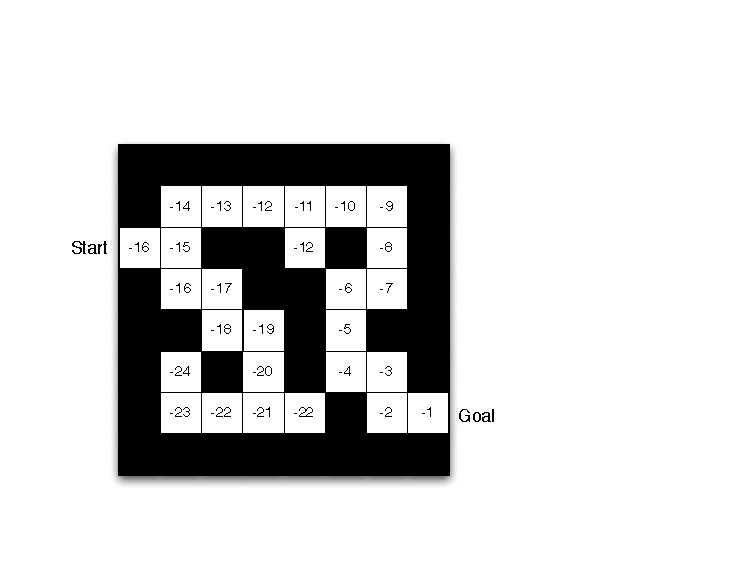
\includegraphics[width=6cm]{fig/lec01/Maze_Value.pdf}
		\caption{Numbers represent value $v_{\pi}(x_k)$ \SilverLectureSource}
		\label{fig:Maze_Value}
	\end{figure}
\end{minipage}
\hfill
\begin{minipage}[c]{0.43\linewidth}
Key characteristics:
	\begin{itemize}
		\item The agent evaluates neighboring maze positions by their value.
		\item The policy is only implicitly available.
	\end{itemize}
\end{minipage}
}

%%%%%%%%%%%%%%%%%%%%%%%%%%%%%%%%%%%%%%%%%%%%%%%%%%%%%%%%%%%%%
%% Maze Model%%
%%%%%%%%%%%%%%%%%%%%%%%%%%%%%%%%%%%%%%%%%%%%%%%%%%%%%%%%%%%%%
\frame{\frametitle{Maze example: RL-solution by model evaluation}
\begin{minipage}[c]{0.55\linewidth}
	\begin{figure}
		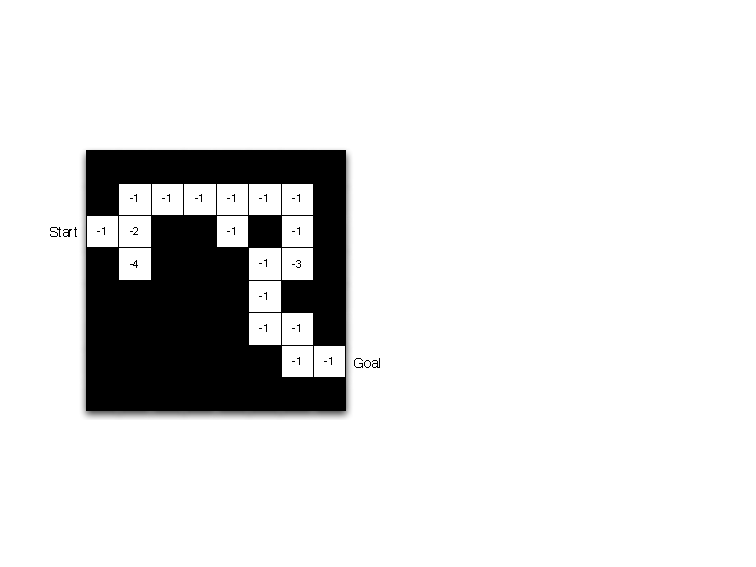
\includegraphics[width=6cm]{fig/lec01/Maze_Model.pdf}
		\caption{Grid layout represents state model $\mathcal{P}$ and numbers depict the estimate by the reward model $\mathcal{R}$.  \SilverLectureSource}
		\label{fig:Maze_Model}
	\end{figure}
\end{minipage}
\hfill
\begin{minipage}[c]{0.43\linewidth}
Key characteristics:
	\begin{itemize}
		\item Agent uses internal model of the environment. 
		\item The model is only an estimate (inaccurate, incomplete).
		\item The agent interacts with the model before taking the next action (e.g., by numerical optimizers).
	\end{itemize}
\end{minipage}
}

%%%%%%%%%%%%%%%%%%%%%%%%%%%%%%%%%%%%%%%%%%%%%%%%%%%%%%%%%%%%%
%% RL Agent Taxonomy%%
%%%%%%%%%%%%%%%%%%%%%%%%%%%%%%%%%%%%%%%%%%%%%%%%%%%%%%%%%%%%%
\frame{\frametitle{RL agent taxonomy}
\begin{figure}
	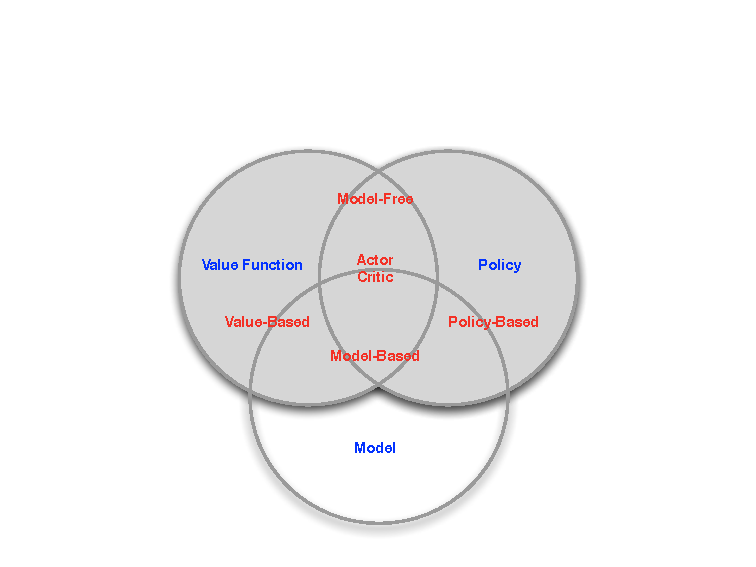
\includegraphics[height=0.7\textheight]{fig/lec01/RL_Agent_Taxonomy.pdf}
	\caption{Main categories of reinforcement learning algorithms\\  \SilverLectureSource}
	\label{fig:RL_Agent_Taxonomy}
\end{figure}
}


%%%%%%%%%%%%%%%%%%%%%%%%%%%%%%%%%%%%%%%%%%%%%%%%%%%%%%%%%%%%%%%%%%
\section{Small comparison to model predictive control} 
%%%%%%%%%%%%%%%%%%%%%%%%%%%%%%%%%%%%%%%%%%%%%%%%%%%%%%%%%%%%%%%%%%
\begin{frame}
\frametitle{Table of contents}
\tableofcontents[currentsection]
\end{frame}

%%%%%%%%%%%%%%%%%%%%%%%%%%%%%%%%%%%%%%%%%%%%%%%%%%%%%%%%%%%%%
%% RL Agent Taxonomy%%
%%%%%%%%%%%%%%%%%%%%%%%%%%%%%%%%%%%%%%%%%%%%%%%%%%%%%%%%%%%%%
\frame{\frametitle{RL vs. planning}
Two fundamental solutions to sequential decision making:
\begin{itemize}
	\item Reinforcement learning:
	\begin{itemize}
		\item The environment is initially unknown.
		\item The agents interacts with the environment.
		\item The policy is improved based on environment feedback (reward).
	\end{itemize}
	\pause
	\item Planning:
	\begin{itemize}
		\item An a priori environment model exists.
		\item The agents interacts with its own model.
		\item The policy is improved based on the model feedback ('virtual reward').
	\end{itemize}
\end{itemize}
\pause
\begin{block}{Remark on learning and planning}
Above the two extreme cases are confronted: 
\begin{itemize}
	\item RL = only learning without using available pre-knowledge.
	\item Planning = iterating on a model without improving it based on data. 
\end{itemize}
\pause
Can this lead to efficient and optimal solutions?
\end{block}
}

%%%%%%%%%%%%%%%%%%%%%%%%%%%%%%%%%%%%%%%%%%%%%%%%%%%%%%%%%%%%%
%% Problem Statement MPC/Rl%%
%%%%%%%%%%%%%%%%%%%%%%%%%%%%%%%%%%%%%%%%%%%%%%%%%%%%%%%%%%%%%
\frame{\frametitle{Problem reconsideration}
The reward hypothesis in \theoref{theo:reward_hypo} is basically an \hl{infinite-horizon optimal control} problem (with $r_k$ interpreted as costs):
\begin{equation}
	v_k^*(\bm{x}_k) = \min_{\bm{u}_k} \sum_{i=0}^\infty r_{k+i+1} (\bm{x}_{k+i}, \bm{u}_{k+i})\,.
\end{equation}
\pause
For certain cases closed-form solutions can be found, e.g., a LTI system with quadratic costs and no further constraints can be optimally controlled by a linear-quadratic regulator (LQR). However, for arbitrary cases that is not possible and one relaxes the problem to a \hl{finite-horizon optimal control} problem:   
\begin{equation}
	v_k^*(\bm{x}_k) = \min_{\bm{u}_k} \sum_{i=0}^{N_\mathrm{p}} r_{k+i+1} (\bm{x}_{k+i}, \bm{u}_{k+i})\,.
\end{equation}
\pause
Here, an internal model $\bm{x}_{k+1}=\bm{f}(\bm{x}_k,\bm{u}_k)$ is utilized to predict the system behavior for $N_\mathrm{p}$ future steps. This \hl{model predictive control} (MPC) approach can be numerically solved. 
}

%%%%%%%%%%%%%%%%%%%%%%%%%%%%%%%%%%%%%%%%%%%%%%%%%%%%%%%%%%%%%
%% Constraints MPC%%
%%%%%%%%%%%%%%%%%%%%%%%%%%%%%%%%%%%%%%%%%%%%%%%%%%%%%%%%%%%%%
\frame{\frametitle{MPC and constraints}
While in RL the desired system behavior must be solely represented by $r_k$, MPC can directly take into account system constraints:
\begin{equation}
	\begin{split}
	v_k^* &= \min_{\bm{u}_k} \sum_{i=0}^{N_\mathrm{p}} r_{k+i+1} (\bm{x}_{k+i}, \bm{u}_{k+i})\, ,\\
	\mathrm{s.t.} \quad\quad \bm{x}_{k+i+1}&=\bm{f}(\bm{x}_{k+i},\bm{u}_{k+i}), \quad \bm{x}_{k+i} \in \mathcal{X},\quad \bm{u}_{k+i} \in \mathcal{U}\,.\\
\end{split}
\end{equation}
\begin{figure}
\centering
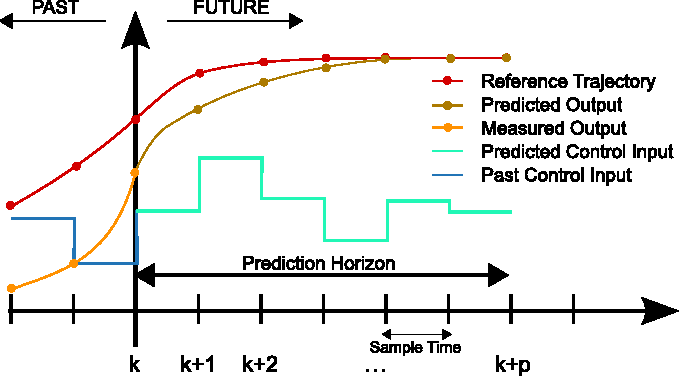
\includegraphics[height=0.4\textheight]{fig/lec01/MPC.pdf}
\caption{Basic MPC scheme (source: \href{https://de.wikipedia.org/wiki/Model_Predictive_Control}{www.wikipedia.org},  by Martin Behrendt \href{https://creativecommons.org/licenses/by-sa/3.0/deed.en}{CC BY-SA 3.0})}
\label{fig:MPC}
\end{figure}
}

%%%%%%%%%%%%%%%%%%%%%%%%%%%%%%%%%%%%%%%%%%%%%%%%%%%%%%%%%%%%%
%% MPC vs RL%%
%%%%%%%%%%%%%%%%%%%%%%%%%%%%%%%%%%%%%%%%%%%%%%%%%%%%%%%%%%%%%
\frame{\frametitle{MPC vs. RL}
\onslide<1->Hence, MPC and RL are two sides of the same coin. Both share the same general goal (\hl{sequential optimal decision making}), but follow their own philosophy:  
\begin{table}
	\centering
		\begin{tabular}{lll}
			Property & MPC & RL\\
			\hline
			\onslide<1->Objective 									& minimize costs 									& maximize return  \\
			\onslide<2->A priori model 							& required \xmark 								& not required \cmark \\
			\onslide<3->Pre-knowledge integration 	& easy \cmark 										& rather complex \xmark \\
			\onslide<4->Constraint handling					& inherent \cmark 								&	only indirect \xmark \\
			\onslide<5->Adaptivity									& requires add-ons \xmark 				&	inherent \cmark \\
			\onslide<6->Online complexity						& it depends \cmark/\xmark		 		&	it depends \cmark/\xmark \\
			\onslide<7->Stability theory						& mature \cmark 									&	immature \xmark \\
		\end{tabular}
	\onslide<1->\caption{Key differences on MPC vs. RL\\(based on D. G�rges, \textit{Relations between Model Predictive Control and Reinforcement Learning}, IFAC PapersOnine 50-1, pp. 4920-4928, 2017)}
	\label{tab:KeyDifferences}
\end{table}
}

%%%%%%%%%%%%%%%%%%%%%%%%%%%%%%%%%%%%%%%%%%%%%%%%%%%%%%%%%%%%%
%% Summary %%
%%%%%%%%%%%%%%%%%%%%%%%%%%%%%%%%%%%%%%%%%%%%%%%%%%%%%%%%%%%%%
\begin{frame}
\frametitle{Summary: what you've learned today}
\begin{itemize}
	\item Understanding the role of RL in machine learning and optimal sequential decision making. \pause
	\item Become acquainted with the basic RL interaction loop (agent, environment, interpreter). \pause
	\item Finding your way around the basic RL vocabulary. \pause
	\item Internalize the significance of proper reward formulations (design parameter). \pause
	\item Differentiate solution ideas on how to retrieve an optimal agent behavior (policy). \pause
	\item Delimit RL towards model predictive control as a sequential decision making alternative. 
\end{itemize}
\end{frame}
